% vim:spell:spl=en_gb:fenc=utf-8:et:sw=4:ts=4:sts=4
%
% This document has been prepared for use with pdfLaTeX 

% The margins produced by standard classes (ar ticle.cls, report.cls, book.cls) 
% are often deemed too wide by Europeans using A4 paper. The classes in the 
% Koma-Script bundle (scrartcl.cls, scrrepr t.cls, scrbook.cls) are specially
% designed for European and German typography (komascript.de):
\documentclass[11pt,bibliography=totoc,index=totoc]{scrbook}   % paper=a4 is default, 11pt is actually also default

% dmthesis.sty : LaTeX style for my Master's Theses
% created by :
%    Dan Michael Olsen Heggø
%    (danmichaelo@gmail.com)

%\typeout{Hello world}

\KOMAoptions{parskip=half, BCOR=7.5mm, DIV=11, mpinclude=false}  % skip margin notes
% DIV=11 gir oss i utg. pkt. 152.73 mm tekstbredde og 216 mm teksthøyde.
% men vi trekker fra 7.5 mm som forsvinner i innbindingen (BCOR)
% og står igjen med 147.26 mm tekstbredde.

\usepackage[greek,british]{babel}		% Localization
\usepackage[utf8]{inputenc}				% For typing accentuated characters directly

%\usepackage{kpfonts}                   % kp is nice for text, but the math isn't acceptable 
\usepackage{lmodern}                    % Use fully scalable fonts
\usepackage[T1]{fontenc}            	% T1 contains the french guillements.. 
\usepackage{lettrine}

%%%%%%%%%%%%%%%%%%%%%%%%%%%%%%%%%%%
% MATH:

\usepackage{amsmath,amsthm,amssymb}		% AMS Math support
\usepackage{empheq,mathtools}
\usepackage{siunitx} 					% For consistent units. Includes upright mu.
										% Must be loaded after amssymb

\renewcommand{\vec}[1]{\boldsymbol{\mathrm{#1}}} 	% Use bold vectors
\newcommand{\nvec}[1]{\mathrm{#1}} 	                % matrices, etc.. 


%%%%%%%%%%%%%%%%%%%%%%%%%%%%%%%%%%%
% FONT:

%\usepackage{kmath,kerkis}          	% The order of the packages matters; 
                                    	% kmath changes the default text font
                                    	% Must be loaded after amsmath

%%%%%%%%%%%%%%%%%%%%%%%%%%%%%%%%%%%
% Figures and tables:

\usepackage[usenames,dvipsnames]{color}	% usenames + dvipsnames gives us 66 predefined colors. 
\usepackage{graphicx}					% Graphicx is the extended graphics package.
%\graphicspath{{imgs/}{moreimgs/}}
\DeclareGraphicsExtensions{.pdf,.png,.jpg} 	% specifies the behaviour of the system when no 
											% file extension is specified in the argument
\usepackage{subfigure} 					% for subfigures

%\usepackage{wrapfig} 					% for \begin{wrapfigure}

% Print figure and table labels in a smaller font, and print `Figure:' and `Table:' in boldface:
\usepackage[margin=10pt,font=small,labelfont=bf,labelsep=colon,format=plain,indention=.5cm]{caption}


\usepackage{booktabs}					% production quality tables
\usepackage{threeparttable}				% for placing footnotes under tables
%\usepackage{multirow} 					% for multi-row table cells

\usepackage{framed} % for drafting only

%%%%%%%%%%%%%%%%%%%%%%%%%%%%%%%%%%%
% CHEMISTRY :

%\usepackage[version=3]{mhchem}			% Latest version: 3.07


%%%%%%%%%%%%%%%%%%%%%%%%%%%%%%%%%%%
% MISC :

\usepackage{fancybox}					% For boxed environments
\usepackage{layout}						% For page layout debug (\layout)
\usepackage{soul}                       % For highlighting (in the draft phase)


% Note that LaTeX can only draw lines with slope = x/y, where x and y have integer values from −6 through 6.
\newcommand{\crossbox}[1]{ %
    \setlength{\unitlength}{#1}
    \begin{picture}(1,1)(0,0)
       \put(0,0){\framebox(1,1){ }}
       \put(0,0){\line(1,1){1}}         % (slope x, slope y){length}
       \put(1,0){\line(-1,1){1}}        % (slope x, slope y){length}
    \end{picture} %
    }



%%%%%%%%%%%%%%%%%%%%%%%%%%%%%%%%%%%
% BIBLIOGRAPHY :
\usepackage[safeinputenc,backend=biber,hyperref=true,sorting=none,style=numeric]{biblatex}


%%%%%%%%%%%%%%%%%%%%%%%%%%%%%%%%%%%
% HYPERREF :
\usepackage{hyperref} 	% Make sure it comes last of your loaded packages, 
						% to give it a fighting chance of not being over-written, 
						% since its job is to redefine many LATEX commands.
						% It is preferable to load it after biblatex.
\hypersetup{pdftex,unicode, 
    colorlinks=true,linkcolor=blue,citecolor=blue,urlcolor=blue,    
    pdfdisplaydoctitle=true, 
    bookmarksopen=true,bookmarksopenlevel=2,        
    pdfauthor   = {Dan Michael Olsen Heggø},            
    pdftitle    = {Not Set Yet},                         
    pdfkeywords = {phosphorus, diffusion, silicon, solar cells, master thesis}
}




\usepackage{makeidx}
\makeindex

% Macros
\newcommand{\ksorb}{\ensuremath{\psi^{\mathrm{KS}}}}

% Temporary premable-stuff:
\usepackage[marginpar]{todo}
\newcommand{\comment}[1]{\hl{#1}}
%\usepackage{layouts}

% Bibliography:
\bibliography{bibliography/master}

% Title page (koma-script options):
%\titlehead{Titlehead}
%\subject{Subject}
%\usepackage{titling}
%\subtitle{Subtitle}
%\publishers{Pub}

\newcommand{\vasp}{{\texttt{VASP}}} % eller \sc?
\newcommand{\vesta}{{\texttt{VESTA}}} % eller \sc?
\newcommand{\vmd}{{\texttt{VMD}}} % eller \sc?

\begin{document}
\frontmatter
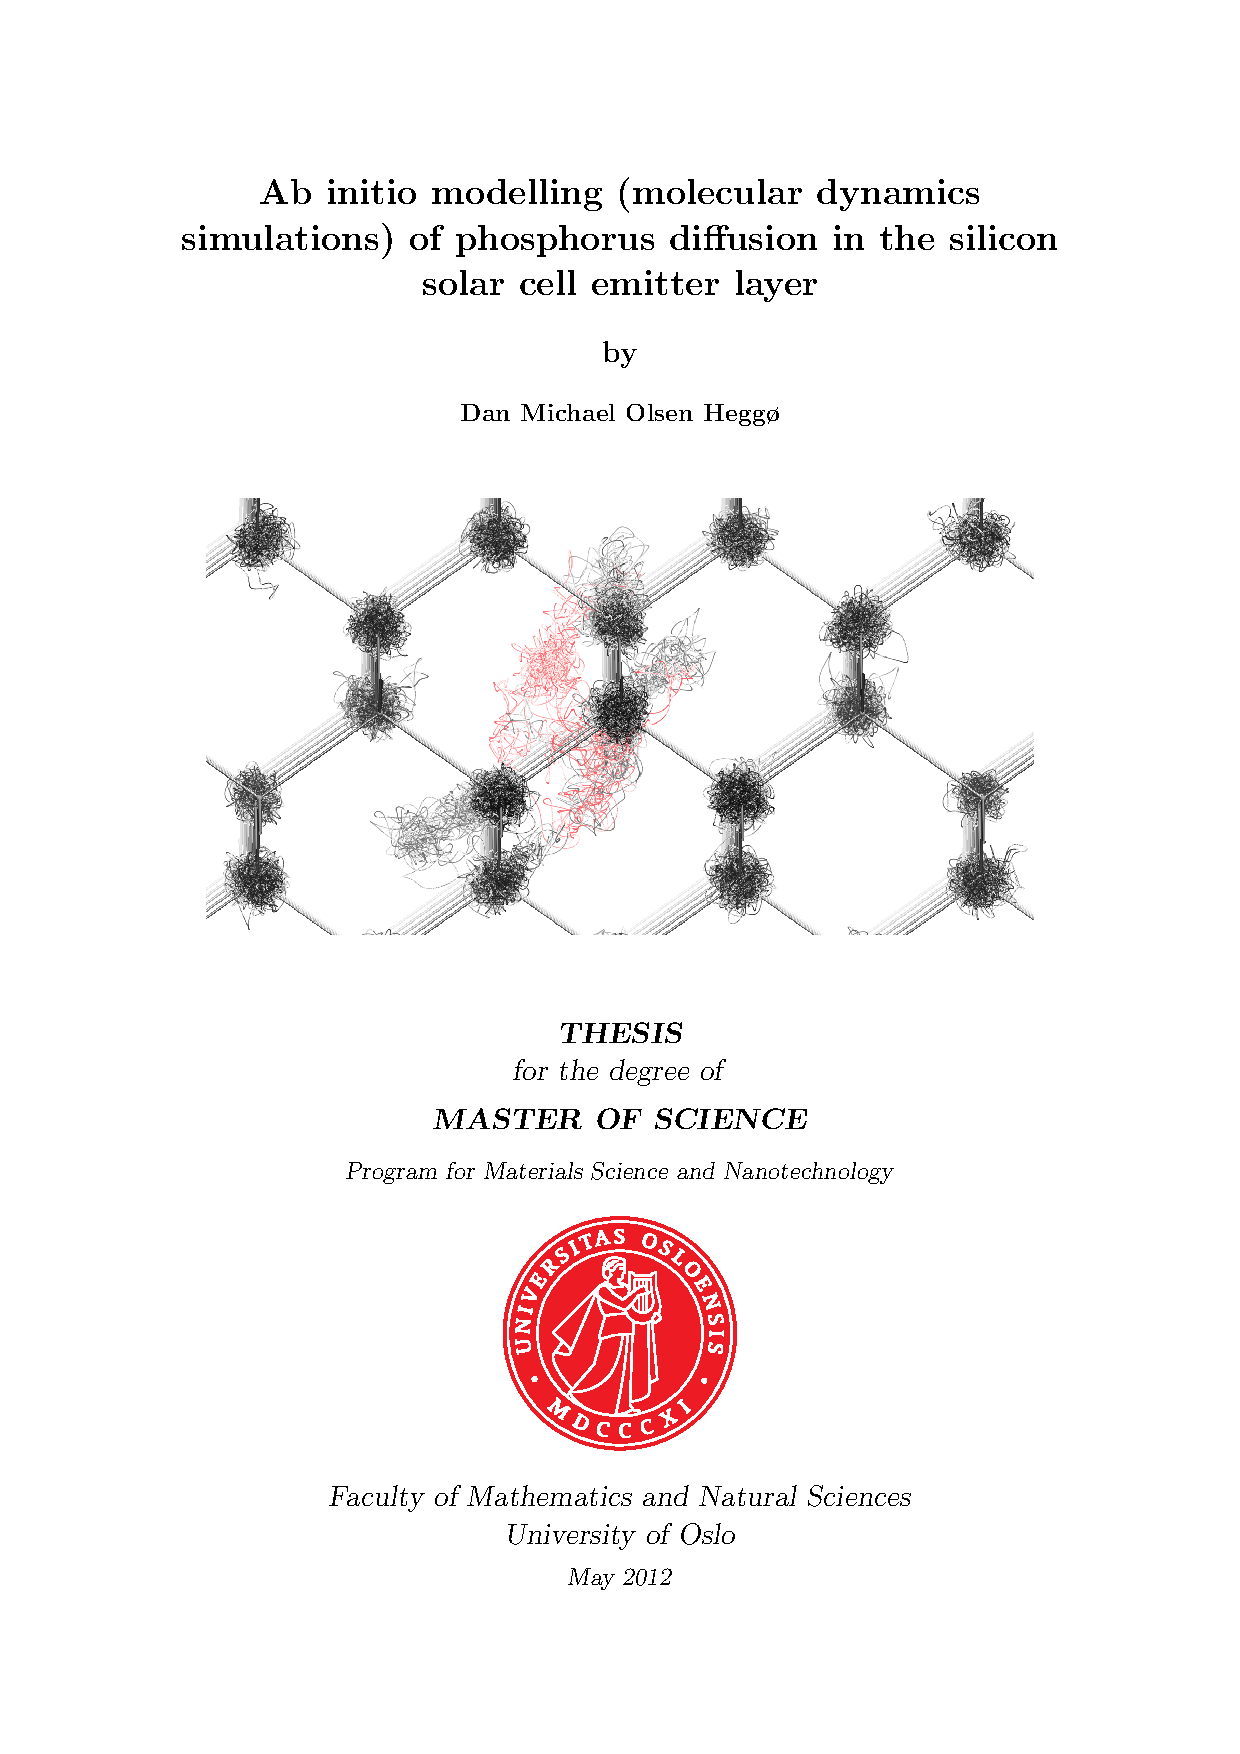
\includepdf{frontpage/frontpage.pdf}

Acknowledgement

Abstract

Sammendrag på norsk

% pdflatex -v | head -n1
Set with the help of {\LaTeXe} and {\KOMAScript}.

%Grasping the amount of work behind this possibility is hard,
%generations before you have laid out the theories of quantum mechanics and of
%solid state physics, prepared a huge library of crystallographic data, 
%developed computing power at a remarkable pace, and written millions of lines
%of computer code. Sometimes you feel very tiny.

\tableofcontents

\mainmatter
\pagestyle{scrheadings}

\part{Background, theory and preparations}

\chapter{Background} % Prolegomena

\section{Introduction}

%\lettrine[lines=3, findent=.2em, slope=-0.5em, nindent=0pt]{W}{hile}
%I personally have no preference for materials over any other matter,
%it happened that I ended up in materials science, the study of 

materials -- ``matter from which a thing is or can be made''\footnote{New Oxford American Dictionary 2nd ed. 2005. I will not 
go into what a `thing' may or may not be.}. 

%I was driven into this discipline by my interest in materials for 

utilisation of some of the \SI{120000}{\tera\watt}
of net power we receive from the Sun -- most of which is `spilled' today. 

Molecular dynamics with an \textit{ab initio} potential, such as one obtained from DFT calculations, is very tempting from a theoretical point of view (finne kilder), but has generally been considered unfeasable from a practical point of view due to the great computational cost involved.
Modeling at the \textit{ab initio}, while 


I'm grateful to the developers of the VASP software, who provided me with new potentials that decreased the computing time considerably. These are described further in section \ldots 

This work was started without knowing \textit{a priori} if simulations at the \textit{ab initio} level could be carried out with simulation times long enough to obtain useful statistics, but with new potentials and \ldots we found it worthwhile to test.

A privilege with studying phosphorus in silicon is that there exists a wealth of experimental and theoretical results from more 
than 60 years\footnote{
  Silicon semiconductor technology took it first infant steps right before world war II, with for instance
  the discovery of the p-n junction (then called `PN barrier') often attribtued to R.S Ohl (U.S. patent 2402662, 1939),
  and the understanding and development gained speed in the early 50s. In a 1953 patent by P. Robsin, the process of 
  diffusion to form a junction is described (U.S. patent 2823149, 1953), and in a 1955 patent by Ross (2862160), 
  phosphorus is mentioned as a donor. But I'm not sure just when phosphorus was first introduced.
} of studies on this system. 
, data that can be used to test our models. 
For example, there are the classic, often-cited reviews on diffusion of dopants in silicon by (Fahey:198) and (Hu:1994). And the PhD thesis of (Bentzen:2006) provides an up-to-date account of the diffusion behaviour of phosphorus in the specific case of the very highly doped emitter layer.

As an introduction, table \ref{tb:si} presents some key properties of silicon,

\begin{table}[htb]
  \centering
  \begin{tabular}{lll}\toprule
     & 300~K & 1100~K\\
     Crystal structure & Diamond  \\ 
     Lattice constant / Å  & 5.43086 \cite{Ghandhi:1994}, 5.43072 $\pm$ 0.00004 Å at \SI{25}{\celsius} \cite{Smakula:1955} \\
     Distance between neighboring atoms / Å & 2.35163 \\
     Atomic density & \SI{4.99441e22}{\per\centi\metre\cubed} \\
     Melting point & \SI{1685}{\kelvin} / \SI{1412}{\kelvin} \\
     Thermal coefficient of expansion & \SI{2.33e-6}{\per\kelvin} & \SI{4.5e-6}{\per\kelvin} \\\bottomrule
  \end{tabular}
  \caption{Some key properties of silicon (Har ikke helt bestemt hvilke som bør være med her)}
  \label{tb:si}
\end{table} 


\section{The power of the sun}
\lettrine[lines=3,slope=0pt,nindent=0pt,lraise=0.12]{Q}uite
stabily, our Sun emits about 383 yottawatts of radiative power [SOURCE]. 
8 light minutes away, our small, blue planet receives about 100 petawatts ($10^{17}$
) of radiative power [CHECK].
In thermodynamic terms, the radiation is an
energy flux of relatively low entropy, meaning that it's easier to utilize
than lower-entropy energy fluxes such as heat. It is a `high-quality' energy
flux, an energy flux that is the starting point for all processes on earth
but those utilising geothermal energy. From a logical point of view, it makes
perfect sense to utilise solar energy directly instead of one of its
`derivates', like wind, hydro, etc. Yet, there is one issue with solar
energy: it's diluted, at least compared with the energy content of fossil
fuels that we are so spoiled with. One litre of gasoline contains about 9.5 kWh of
energy\footnote{\url{http://www.ocean.washington.edu/courses/envir215/energynumbers.pdf}}.

To get a feeling for this number, remember that one kilowatt-hour of electric power 
is roughly one and a half hour of horse-power. Man, not being as strong as a
horse, can only sustain about one tenth of a horsepower over time, meaning that a 
full working day amounts to less than one kilowatt-hour, further meaning that 
roughly 10 hard working days can be replaced by a single litre of gasoline in terms
of energy content. 

How about solar power? In a solar-rich area, we receive the same amount of energy 
over 9.5 square metres in one hour. That's why we say that solar power is rather
\emph{area-intensive}.

Blabla. solceller må derfor være tynnest mulig og mest mulig effektiv.

solar constant: 

$1366\pm 40$ W/m$^2$. The yearly variation of about $\pm 3\%$ 
due to the variation of Earth's distance to the Sun during the year, is much
larger than the known variations in the radiation itself.\footnote{
Phillips, Kenneth J. H. (1995). Guide to the Sun. Cambridge University Press. 
pp. 14–15, 34–38. ISBN 9780521397889.
\url{http://www.pmodwrc.ch/pmod.php?topic=tsi/composite/SolarConstant}
\url{http://books.google.com/books?id=YEN9fC9tbEgC}
}

solar constant $1353\pm 45$ W/m$^2$ (Marstein forelesningsnotater)
. de Vos, s. 19: 1353, pm 3.5\%.

About $5.8\times 10^{17}$ photons/sec/cm$^2$ reach the outer atmosphere, while
some $10^{17}$ survive through the atmosphere.\footnote{Solar Cells (Backus)}

\section{The silicon solar cell}

Silicon doped with a donor, like phosphorus, is called n-Si. Highly-doped areas in the proximity of the metal contacts are often referred to as n+ or n++.

The contact resistivity $\rho_c$ depends strongly on the doping concentration $N_D$, as reviewed by Schröder\cite{Schroder:1984}. 
If the metal contacts take up 5\% of the cell surface, a contact resistance $\rho_c < \SI{2e-3}{\ohm\centi\metre\squared}$ is required to not degrade the output power by more than 0.5\%. This in turn requires a doping concentration $N_D > \SI{1e19}{\per\centi\metre\cubed}$,but even higher doping concentrations is required if the area occupied by metal contacts is reduced, or if used in concentrator cells with higher power.

\subsection{Short solar cell history (kan kanskje sløyfes)}

The ``Effect of Light on Selenium during the passage of an Electric Current''
was described by W. Smith in 1873\cite{Smith:1873}.

1876 eller 1877 (?) - W.G. Adams and R.E. Day observed the photovoltaic effect in solidified 
selenium, and published a paper on the selenium cell. 'The action of light 
on selenium,'\cite{Adams:1876}

The first known solar cell was built in 1883 by Charles Fritts who coated the
semiconductor selenium with a thin layer of gold to form a junction.

Russell Ohl, in 1939, discovered the PN barrier (or as it became known, 
the “P–N junction”). He is generally recognized for patenting the modern solar 
cell (US Patent 2402662, "Light sensitive device"). Ohl was a notable 
semiconductor researcher prior to the invention of the transistor. 

Solar cells later became practical for power uses after Russell Ohl's 1941 
development of silicon p/n junction cells that reached efficiencies above 
5\% by the 1950s/1960s.

%Multicrystalline silicon (mc-Si) wafers are widely used for man- 
%ufacturing of solar cells due to their relatively low price and high 
%performance. is responsible for the kink-and-tail profile [11–13]. The effective 
%diffusivities describing the high and low concentration regions of 


%Today, silicon-based solar cells are most widely used because of their
%relatively low price and high performance. Even cheaper are many of the thin
%film approaches, but at the cost of lower performance, meaning larger areal
%cost. The most popular also make use of scarce elements, which mean that such
%solar cells cannot play a major part of a renewable energy scenario.

%While solar cells today are commonly quoted as being to expensive, a remarkable
%project initiated by the Barefoot College in India have shown that even the
%poorest of the poor can often reduce their expenses by replacing kerosene with
%silicon solar cell based lightning.

%The main problem is of course that fossil fuel is underpriced.

%Even so, there is a broad hope for a great increase in solar cell performance in
%the coming years. How is it to be achieved? From a modelling point of view we
%can study both materials that have never been tested in the real world. Can
%computer modelling give us insight into what the ideal solar cell material would
%be?


\section{Diffusion and diffusivity}

Diffusion\index{diffusion} is the redistribution of atoms\footnote{I will only be concerned with atoms here, but the concept of diffusion also applies to other small particles such as molecules, viruses and bacteria} due to their thermal motion. 
Such redistribution occurs in all materials, but at a negligible rate at temperatures considerably below the melting point of the material.
For silicon, with a melting point of \SI{1414}{\celsius}, diffusion is negligible at room temperature, 
but significant at elevated temperatures, and controlled diffusion is commonly carried out at temperatures 
of about 800-\SI{1000}{\celsius}. 

How do we describe and model diffusion?
As is not uncommon in physics, different pictures exist for different scales of interest. 
When it comes to describing diffusion, two main pictures exists: the continuum picture and the atomistic picture. 
Since materials consists of atoms, it is clear that the most fundamental picture of diffusion should be an atomistic one.
But a description involving every single atom becomes highly impractical on a macroscopic scale\footnote{\comment{Clarify macroscopic / microscopic?}
}, in which it becomes more practical to invoke a viscous fluid model in which the atoms are smoothed out into a continuum.
The two pictures can be connected through parameters known as diffusion coefficients in order to produce integral diffusion models,
but the diffusion coefficients are also commonly obtained empirically.

\subsection{The continuum picture}

Following Joseph Fourier's 1822 treatise on heat diffusion\cite{Fourier:1822} and Georg Ohm's 1827 work on `electricity diffusion' (Ohm's law),\cite{Ohm:1827} Adolf Fick presented his phenomenological description of `mass diffusion' in 
1855.\cite{Fick:1855}
In this picture, a species with concentration $c(\vec{r})$ will flow in the opposite direction of the concentration gradient of that species, $\nabla c(\vec{r})$. That is, it will show a flux,
\begin{equation}
  \vec{J}(\vec{r},t) = - D \nabla c(\vec{r},t).
  \label{eq:ficks1st}
\end{equation}
This relationship between the concentration gradient and the flux is known as Fick's first law, and the constant of proportionality $D$ is known as the coefficient of diffusion or \emph{diffusivity}\index{diffusivity} for the species in question. 
Often reported in units of \si{\metre\squared\per\second} or \si{\centi\metre\squared\per\second}, the diffusivity is in general a tensor, but it reduces to a scalar in cubic crystals. 
In general the diffusivity of species $i$ will depend on both the concentration of the same species $c_i$ and of other species $c_j$, on temperature, pressure, crystal defects and other factors that will be quickly discussed below.

If $G$ and $R$ are the generation and recombination rates for the species in question, a continuity equation could be set up as
\begin{equation}
    \frac{\partial c}{\partial t} = -\nabla \vec{J} + G - R
  \label{eq:continuity}
\end{equation}
In the absences of sinks and sources ($G=R=0$), the continuity equation combined with Fick's first law forms what is known as Fick's second law,
\begin{equation}
    \frac{\partial c}{\partial t} = \nabla (D \nabla c) = D \nabla^2 c
  \label{eq:ficks2nd}
\end{equation}
where the last equality is true only when $D$ is independent of position (via the concentration).

The picture is slightly complicated by the fact that the diffusivity $D$ itself may vary with the concentration $c$.
\index{diffusivity!dependence on concentration}
For the diffusivity of species at very low concentrations, such as dopants, this concentration dependence is generally negligible, but at high concentrations, such as the typical phosphorus concentrations in the solar cell emitter layer, the effect may be quite significant.
As an example, A. Bentzen has obtained the concentration dependence of the phosphorus diffusion coefficient over a large range of concentrations using Boltzmann-Matano analysis of experimental data at \SI{890}{\celsius}. 
From the intrinsic value of about \SI{4e-14}{\centi\metre\squared\per\second}, his diffusivity increases slowly up to a maximum of \SI{1e-13}{\centi\metre\squared\per\second} at a phosphorus concentration of \SI{e19}{\per\centi\metre\cubed}, before it dips down to \SI{1e-14}{\centi\metre\squared\per\second} at \SI{e20}{\per\centi\metre\cubed}, before it increases again.\cite{Bentzen:2006} Concentration gradients will nevertheless not be considered in this work.\comment{upresist?}

\index{diffusivity!dependence on temperature}
The diffusivity depends strongly on the temperature, and the temperature dependence found from experiments often takes the simple Arrhenius form,
\begin{equation}
  D(T) = D_0 e^{-E_a/kT}
\end{equation}
defined by a prefactor $D_0$ and an activation energy $E_a$. 
Taking the logarithm on both sides, we see that $\ln D$ as a function of $1/kT$ forms a straight line with slope $-E_a$ and interceipt $\ln D_0$. 
\begin{equation}
  \ln D = \ln D_0 - E_a (kT)^{-1}
\end{equation}
The parameters $D_0$ and $E_a$ can thus easily be extracted if a good fit can be made to a straight line.

%While diffusion is an activated process, the activation energy obtained from experiments will in general not result from a single activated process, but rather a mix of different processes, and this necessarily complicates the determination of the processes involved.
%In fortunate cases, a single process may be dominating.

%Since the diffusion of atoms in an crystal is though of as an activated process with an activation energy $E_a$, the temperature dependence will often take the simple Arrhenius-form,

As mentioned, the diffusivity may also depend on other factors, such as crystal defects, pressure, et cetera, that will not be touched upon in this work, but these are discussed by e.g. Pichler.\cite{Pichler:2004}

\subsection{The atomistic picture}

In the continuum picture, the diffusion coefficients are just empirical parameters, and we have to invoke a model involving atoms to explain them.

From the Gaussian diffusion outwards from a point,
\begin{equation}
    c(x,t) = \frac{n}{\sqrt{4\pi D}} e^{-x^2/4Dt} / \sqrt{t},
\end{equation}
\comment{SJEKK OPP}
Einstein related the displacement along the $x$ axis, $\lambda_x$, to the diffusivity\cite{Einstein:1905},
\begin{equation}
    \lambda_x = \sqrt{x^2} = \sqrt{2Dt}
  \label{eq:einsteinRelationSimple}
\end{equation}
Na\"{\i}vely, the diffusion coefficient of a species can thus be found from a knowledge of the displacement of all atoms of that species,
and this is actually the approach followed in molecular dynamics simulations.
While it's a tempting approach, and also the one followed in this work, it should not come to a surprise that simulating a large number of atoms over a sufficient amount of time is a computationally demanding task, and for many systems it's just not feasible. 
A short discussion of other approaches is therefore in place, especially since these to a large degree have formed the way we understand and describe diffusion.

In the solid phase, very little diffusion occurs compared to the liquid or gas phase. 
In a crystal, the atoms remain at given lattice sites most of the time.
At a finite temperature $T$, the atoms will have kinetic energies according to a Boltzmann distribution for that temperature,
and since the atoms are `trapped' by the neighbouring atoms this energy goes into vibrations. 
If, however, an atom obtain a kinetic energy larger than a given treshold energy, it can migrate (`jump') into another site.
This is an example of what is called an \emph{activated process}, and the treshold energy is called an activation energy, $E_a$.
In general there is not just one diffusion mechanism involved, and the value for the activation energy obtained by experiment or simulation is a weighted average over all possible mechanisms.
One mechanism may, however, be the dominating one. In the case of phosphorus in silicon, there is a general consensus that interstial-mediated diffusion is the dominating mechanism. \comment{KILDER!}

Now, from the Boltzmann distribution (see \ldots), the fraction of atoms having a kinetic energy greater than a given energy $E_a$ is $e^{-E_a/KT}$, and so the probability for a jump to happen is just $e^{-E_a/kT}$. 

In a simple model, we can estimate the number of jumps per second \comment{PER ATOM?} by multiplying this probability by the attempt frequency $\nu$,
\begin{equation}
  \Gamma = \nu e^{-E_a/kT}
  \label{eq:jumpfreq-est}
\end{equation}
For a rough estimate, we may take the frequency to be \SI{e13}{\hertz}, a typical textbook value for the vibration of atoms in a crystal at room temperature.
As seen in fig. \ref{fig:simple-vibration}, the atoms may be described roughly as vibrating at frequencies of this order of magnitude, although the motion is of course much more complicated than a simple harmonic motion. Otherwise we would not need \emph{simulation}.

\begin{figure}[htbp]
  \begin{center}
    \includegraphics{../figures/md_test_fft}
  \end{center}
  \caption{
    Simulated motion of a silicon atom in a 64-atom supercell at 1400 K (solid line), 
    with a least square fit to a function $f(t) = a \cos[(2\pi f)t + c] + d$ (dashed line). 
    The fitted frequency is $f=\SI{3e12}{\hertz}$, corresponding to a period of 0.3~ps.
  }
  \label{fig:simple-vibration}
\end{figure}

\begin{figure}[htbp]
  \begin{center}
    \includegraphics{../figures/jump_frequency}
  \end{center}
  \caption{Estimated jump frequency from \eqref{eq:jumpfreq-est} with $\nu=\SI{e13}{\hertz}$.}
  \label{fig:jumpfreq-est}
\end{figure}




At the microscopic scale, an atom in a crystal will not move freely, but vibrate in a unharmonic and complicated way in the potential well of the other atoms. 
If its motion is averaged over the timescale of the vibrations, which are in the order of pico-seconds, it will appear more or less fixed in space. 
Every now or then, it will, however, obtain enough energy to `jump' to a different position.

\begin{figure}[htbp]
  \begin{center}
    \includegraphics{../figures/md_test_diffusion_jump}
  \end{center}
  \caption{A `jump' from one lattice site to another. The red line is a symmetric running mean over 0.5 ps followed by a symmetric running median over 2.0 ps.}
  \label{fig:../figures/md_test_diffusion_jump}
\end{figure}

The diffusion coefficient in liquids is typically of the order of $10^{-7}$ cm2/s,
while in solids its magnitudes smaller, typically of the order of $10^{-11}$ cm2/s. \comment{[kilder!]}


The diffusion coefficient in crystals with a cubic lattice should be isotropic.

\section{The case of phosphorus diffusion in silicon}\label{sec:PinSi}

The atomic radii of silicon and phosphorus are 1.17 and 1.10~Å, respectively.
A solid solution of phosphorus in silicon is therefore expected to have a slightly smaller lattice parameter than pure silicon.
That a small shrinkage takes place on in-diffusion of phosphorus into silicon was first described by Pearson and Bardeen in 1948, who reported a slight lattice constant shrinkage of some 0.02 \% when adding some 0.5 at\% phosphorus,\cite{Pearson:1949} 

Comparing Pauling's tetrahedral covalent atomic radii (Kittel, p. 105), $(V_{\text{Si}}-V_{\text{P}})/V_{\text{Si}} = -0.17$.
Using effective-mass theory, Pajot and Stoneham found a volume contraction, $\Delta V/V_{\text{Si}} = -0.08$.

The solid solubility of phosphorus is in the order of 1\%. After in-diffusion of phosphorus into silicon , an annealing step 
After proper annealing, the density of electrically active dopants can reach about 2–\SI{3e20}{\per\centi\metre\cubed}, or 0.4--0.6\%,
or even \SI{4e20}{\per\centi\metre\cubed} for annealing temperatures higher than those used in normal solar cell processing.

but at temperatures above \SI{750}{\celsius}, 
however, the limit of solunlieven more phosphorus appears to be solv

Newero\cite{Borisenko:1987} and \cite{Safarian:2011} 

According to the standard phosphorus-silicon binary phase diagram, more than 2\% P can be solved in silicon at temperatures at temperatures between \SI{1350}{\kelvin} and \SI{1500}{\kelvin} without the formation of new phases, and even at 1000 K about half a percent can be solved.\cite{PSiPhaseDiagram} 
Sheet resistivity and Hall effect measurements have shown that below about 2–\SI{3e20}{\per\centi\metre\cubed} (or 0.4-0.6\%), the density of electrically active dopants in properly annealed samples follow the chemical concentration of phosphorus closely, but above such a concentration, the density of electrically active dopants $n_e$ plateau.\cite{Tannenbaum:1961}
A concentration of about half a percent therefore seems to be the maximum solubility of unclustered P,\cite{Solmi:1998} but higher concentrations
%(reached above about \SI{750}{\celsius},\cite{Solmi:1996} and)
are common in the heavily doped emitter layer in solar cells.\cite{Bentzen:2006b}
The exact nature of the ``extra'', inactive phosphorus is not known, but a mix of SiP precipitates and mobile P defects have been suggested.\cite{Armigliato:1976}\cite{Solmi:1996} 
%When the concentration of phosphorus exceeds the solid solubility,  orthorhombic crystallites of silicon monophosphide (SiP) will start to precipitate within the silicon matrix,\cite{Arimgliato:1976} 

\chapter{Density Functional Theory}

Note to self: In DFT, the electron density is usually denoted $n(\vec{r})$ or
$\rho(\vec{r})$. I think $n$ may be the more common choice, but that conflicts
with $n$ as the free carrier density in semiconductor theory. Are we using
$\rho$ somewhere?

``What are the electrons really doing in molecules?''\footnote{What are the
Electrons Really Doing in Molecules? \textit{The Vortex}, Cal. Sec. of
Am. Chem. Soc., Spring, 1960.}

\section{Describing materials (bør antakelig kortes ned)}

%\lettrine[lines=3,slope=0pt,nindent=0pt]{M}{aterials} can be described and 
As touched upon in section \ldots, matter can be described in different pictures. When radioactivity is not of interest, we are usually not interested in what happens within the nuclei, but rather the interaction between nuclei and electrons, from which chemical bonding and almost all material properties can be understood to the accuracy of interest (with higher accuracy taking longer time to calculate).

%most cases of interest within the atomistic picture. 
%modelled accurately enough for 
%in 
%can be modelled very accurately by considering it
%as large collections of positive nuclei and 
%negative electrons, and we call the 

As de Broglie first hypothesised in 1924,\cite{deBroglie:1924} matter has wave
properties. Quantum effects become important when the average inter-particle
separation is of a size comparable to or smaller than the de Broglie wavelength 
of the particle.\footnote{\url{http://cmt.dur.ac.uk/sjc/thesis_ppr/node5.html}. [Finn
en bedre kilde!}. The de Broglie wavelength of an electron is $\lambda=h/p$.
Using the classical energy-momentum relation $E=p^2/2m$, we obtain
\begin{equation}
  \lambda = \frac{h}{p} = \frac{h}{\sqrt{2m_eE}} 
  \label{eq:deBroglieWavelength}
\end{equation}
For a free electron, the thermal energy $E\sim kT$, 
giving $\lambda\sim\SI{77}{\angstrom}$ at
room temperature. In comparison, the lightest element, hydrogen, has thermal
energy $E\sim\frac32 kT$ and 
$\lambda\sim\SI{1.5}{\angstrom}$. While atoms as a whole generally can be 
threated classically, quantum effects do have some practical effects on them.
For instance, many chemical reactions involving hydrogen, carbon and oxygen 
proceeds much faster because of tunneling. In the molecular dynamics simulations, 
a combination of the classical and quantum mechanical pictures will be used, as 
described below, but tunneling will be negligible for the rather heavy elements 
of interest; silicon and phosphorus.

For solid-state systems, the average separation between two non-interacting
electrons can be roughly estimated by the Wigner-Seitz radius $r_s$, 
which is the radius of a sphere whose volume encloses a single electron

If the average electron density is $\rho$, then one electron occupies a volume
$1/\rho$. If we assume this volume is spherical, the average distance between
two electrons is two times the radius of this sphere\footnote{This is a
typical back-of-the-envelope type calculation.}, often termed the 
Wigner-Seitz radius\footnote{Phys. Rev. 43, 804 (1933)},
\begin{equation}
  \frac43\pi r_{wz}^3 = \frac{1}{\rho}\quad
  \Rightarrow \quad r_{wz} = \left(\frac{3}{4\pi\rho}\right)^{1/3}
  \label{eq:wigner-seitz}
\end{equation}
For typical materials, $r_s$ is of the same order of magnitude as $\lambda$. The
de Broglie waves overlap and a quantum mechanical treatment is necessary.

The thermal wavelength for an ideal gas is
\begin{equation}
  \Lambda = \frac{h}{\sqrt{2\pi m k_B T}} \approx \frac{\SI{18}{\angstrom}}{\sqrt{A_r T}}
\end{equation}
where $A_r=m/m_u$ is the (dimensionless) relative atomic mass with
$m_u\approx\SI{1.66e-27}{\kilogram}$ as the atomic mass constant.
$T$ is the temperature in Kelvin.
We see that for very light atoms at very low temperatures, quantum
effects becomes important, but for most atoms at normal temperatures they are not.
The relative atomic mass of the electron, however, is about $1/1800$, so 
electrons must be described quantum mechanically

In quantum mechanics, the system is fully
described by the concept of a quantum state $|\Psi\rangle$. The state (or
states) with the lowest energy is called the \emph{ground state} (GS), 
while the other states are called excited states. We extract information about 
observables like energy, momentum, \textit{et cætera} from the state by 
letting Hermitian linear operators act on the state. As an example, the 
kinetic energy of a particle $i$ is the expectation value of the kinetic 
energy operator
\begin{equation}
  \hat{T}_i = -\frac{\hbar^2}{2m_i}\nabla_i^2.
  \label{eq:kineticenergy}
\end{equation}
The energy of a state is the expectation value of an energy operator (A
Hamiltonian $\mathcal{H}$) consisting of terms describing the kinetic 
energy\footnote{Since quantum mechanical particles do not follow \emph{trajectories} 
in the way classical particles do, the name `kinetic energy' is 
a bit misleading, Reflecting the spatial variation of the wavefunction, Sauer and Kuhn suggested the 
name `localization energy' instead for this term\cite{Sauer:1982}.
Yet, with the close analogy with classical kinetic energy, we will continue to use that name.
}
and the potential energy arising from interactions with other particles.
Terms describing relativistic and magnetic effects may be included.
If the state of interest is the ground state, we find the ground state energy.
[\dots] At each point in space $\vec{r}$, the quantum state can be represented by a 
wavefunction $\Psi(\vec{r})=\langle\vec{r}|\Psi\rangle$.



\lettrine[lines=3,slope=0pt,nindent=0pt]{S}{ome}
of the first tests of quantum mechanics were optical measurements of
isolated atoms (i.e. gases), which resulted in spectra with sharp, narrow 
lines interpreted as resulting from transitions between the allowed energy 
levels. Predicting and interpreting the broad spectra obtained from condensed 
matter, although they also contained definitive electronic structure, required 
far more sophistication. In the early 1960s, high quality energy level diagrams 
(band diagrams) was calculated for silicon and germanium with the aid of a few
parameters determined from optical experiments, using the empirical
pseudopotential method\footnote{JC Philips, L Kleiman. Phys. Rev 116, 287
(1959), MH Cohen, V. Heine. Phys. Rev. 122, 1821 (1961).}. While such
empirical approaches have been very important for our understanding of
semiconductors, it has been a major aspiration of condensed matter
physics to explain and predict the properties of solids from `first
principles', knowing only the identities of the constituent
atoms\footnote{Cohen, Chelichowsky. Electronic structure and optical
properties of solids. Introduction.}. Today this goal has been reached for
most of the properties of pure semiconductors, and more realistic
semiconductors involving defects are also studied. While some calculations
are straightforward today, many are still not. This includes calculations of
materials with highly correlated or localised electrons, and the calculation
of excited state properties among others.

Still, electronic structure software can today be downloaded from the
internet to your home, sometimes for free, where it can run calculations 
not thought possible a few
decades ago. 

\section{The many-particle problem and the Born Oppenheimer approximation}\label{sec:born-oppenheimer}
\comment{Skille mellom adiabatisk og BO eller ikke?}

Our system of interest consists of a large number of nuclei and electrons, particles whose motion are correlated by their Coulombic interactions. 
While there is no known way to describe the mutual interaction of many particles in general, the reductionist principle of physics leads us to describe it as a sum of two-particle interactions between particles, for which simple equations exist.\footnote{
Such a description is usually a very good one for particles interacting by relatively weak forces such as gravitational forces or Coulomb forces, but a description of particles interacting by strong nuclear forces requires the inclusion of at least three-particle interactions.}
With this approach we can set up equations describing the motion of a general system of many particles, with `many' now meaning `more than two', but we can not solve the correlated equations exactly (analytically) even when using the relatively simple Newtonian equations of classical mechanics. 
This is the `many-particle problem' or `many-body problem', perhaps first encountered by Newton as he studied the three-body problem of the motion of the Earth-Moon-Sun system interacting gravitationally.\footnote{Principia, Book 1, section XI, Proposition 66 and its corollaries,
\url{http://en.wikisource.org/wiki/The_Mathematical_Principles_of_Natural_Philosophy_(1729)/Book_1/Section_11\#Prop66}
\url{http://books.google.com/books?id=ySYULc7VEwsC&pg=PA173}
(Newton, 1687, english transl. by Motte 1729) 
The problem received great attention, as exemplified by the two-volume work La Théorie du mouvement de la lune, 1800 pages in length, published in1860 and 1867 by Charles-Eugène Delaunay on the system.}
Approximate solutions to the Earth-Moon-Sun system can be found quite easily. 
Due to the large mass difference between the three `particles' the problem can be decoupled into the Earth-Sun and the Earth-Moon problems.
Interactions with the other planets may also be ignored successfully at first.

Similarly, the quantum-mechanical two-body problem of a single electron interacting with a single nuclei is solvable, while the introduction of more particles makes approximate numerical solutions necessary. 
And with the electron being 1800 times lighter than the lightest nuclei, the hydrogen nuclei, approximate solutions may be found by decoupling the motion of the nuclei and the electrons. 
This is the central idea of the Born Oppenheimer approximation\cite{BO:1927}.

To put this in a mathematical language, a system of $N$ electrons and $M$ nuclei can be described in Hartree atomic units\footnote{SJEKK
in which the electron mass $m_e$, the elementary
charge $e$, the reduced Planck constant $\hbar$ and the Coulomb constant
$k_e$ all are unity by definition.
} by the Hamiltonian (foreløpig IKKE i atomære enheter)
\begin{align}
  \hat{H} &= 
	 \underbrace{
		- \frac{\hbar^2}{2}\sum_{k=1}^M \frac{1}{m_k}\nabla_k^2 
        + k_e \sum_{k<l}\frac{e^2Z_kZ_l}{r_{kl}}
		}_{\text{nuclei}}
  +
  \underbrace{
	-\frac{\hbar^2}{2}\sum_{i=1}^N\frac{1}{m_e}\nabla_i^2
	+ k_e  \sum_{i<j}\frac{e^2}{r_{ij}}
	}_{\text{electrons}}
		+ k_e \sum_{i=1}^N\sum_{k=1}^M \frac{e^2Z_k}{r_{ik}}
  \label{eq:mol-hamiltonian}
\end{align}
with the first two terms representing the kinetic energy of nuclei and electrons, respectively, 
and the last three terms representing nuclei-nuclei interactions, electron-electron interactions
and nuclei-electron interactions, respectively.
The indexes $i$ and $j$ runs over all electrons, while $k$ and $l$ runs over all nuclei. 

As seen, only electromagnetic (Coulombic) interaction is included. 
The particles also interact gravitationally, but this can safely be ignored since the gravitational force is so much weaker than electromagnetic one.\footnote{Remember that a small kitchen magnet counteracts the gravitational pull of the entire Earth.}
At the atomic scale, gravitation is completely negligible. But there are
other terms we could include in the Hamiltonian, like interaction with external electric or magnetic fields, spin coupling terms, etc.

While the many-body problem prevents exact analytic solutions, solutions to any given accurancy can be found from iterative, numerical methods, only limited by numerical accuracy and computational power. Computational power is a severe practical limitation though, and even with quite drastical approximations involved, it limits us to study systems of roughly a few thousand atoms. Computational power increase rapidly, and in 10 years, we may study tens of thousands of atoms, but still we will be far away from, say, the $10^{22}$ atoms in a gram of salt.

%\section{The Born-Oppenheimer approximation}

The reduction from a fully quantum description to a classical potential entails two main approximations. The first one is the Born-Oppenheimer approximation, which states that the dynamics of electrons is so fast that they can be considered to react instantaneously to the motion of their nuclei. As a consequence, they may be treated separately. The second one treats the nuclei, which are much heavier than electrons, as point particles that follow classical Newtonian dynamics. In classical molecular dynamics the effect of the electrons is approximated as a single potential energy surface, usually representing the ground state.

The mass of a proton or a neutron is about 1800 times the mass of an electron.
Since the nuclei are so much heavier than the electrons, they will move much
slower. In the Born-Oppenheimer approximation, the motion of the 
nuclei and
electrons are de-coupled: we assume that the electrons update their positions
instantaneously for a given placement of the nuclei, and we can compute
electronic energies for fixed nuclear positions. This gives us the so-called
\emph{electronic} Hamiltonian, which only includes terms involving the
electrons,
\begin{equation}
  \hat{H}_e = 
	k_e  \sum_{i<j}\frac{e^2}{r_{ij}}
	-\frac{\hbar^2}{2}\sum_{i=1}^N\frac{1}{m_e}\nabla_i^2
		+ k_e \sum_{i=1}^N\sum_{k=1}^M \frac{e^2Z_k}{r_{ik}}
  \label{eq:el-hamiltonian}
\end{equation}
The expectation value of this Hamiltonian plus the (constant) nuclear-nuclear 
repulsion energy $V_N$ is the \emph{electronic energy}, which
is now a parametric function of the nuclear coordinates. The Born-Oppenheimer
approximation is fundamental in most electronic structure methods, including
DFT. Further references to the Hamiltonian in this chapter will implicitly 
be to the \emph{electronic} Hamiltonian unless otherwise stated. 
We will return to the nuclei Hamiltonian in chapter \ref{cha:molecular-dynamics}



The Born-Oppenheimer approximation is justified in most 
cases,\cite[p. 111]{Cramer:2004} but it should not be applied blindly.
The common phenomena of Joule heating, for instance, utilitised in everyday electrical heating appliances, can not be described using the approximation, since it involves electrons dissipating energy into ionic vibrations, coupling the motion of the electrons and the nuclei.\cite{Horsfield:2004b}

We start by splitting the total Hamiltonian $\hat{H}$ into a so-called `electronic Hamiltonian' $H_e$ and a `nuclear Hamiltonian' $H_n$, with
\begin{equation}
  \hat{H}_e = \hat{H} - \hat{T}_n - \hat{V}_{nn} = \hat{T} + \hat{V}_{ee} + \hat{V}_{ne}
\end{equation}

The full wavefunction $\Psi$ depends on the set of electron coordinates $\vec{x}=\{\vec{x}_i\}$, the set of nuclear coordinates $\vec{R}=\{\vec{R}_i\}$ and the time $t$.
We start by expanding it into a complete set of functions $\Phi(\vec{x}\;\vec{R})$,
\begin{equation}
  \Psi(\vec{R},\vec{x},t) = \sum_n \Theta_n(\vec{R},t)\Phi_n(\vec{x}\;\vec{R})
\end{equation}
where 
The 

The full wavefunction of the system can be expanded in the complete set of adiabatic electronic eigenstates $\Phi(\vec{x}\;\vec{R})$
where the \emph{parametric} dependence of $\Phi$ on $\vec{R}$ is indicated by the semicolon.

The BO accounts to
\begin{equation}
  \Psi(\vec{R},\vec{x},t) = \Theta_n(\vec{R},t)\Phi_n(\vec{x}\;\vec{R})
\end{equation}

\section{The exchange-correlation hole}

The electronic density $\rho(\vec{r})$ is the probability that any one electron will be located in a small volume $d\vec{r}$ 
around $\vec{r}$.
Now, the probability of finding electron 1 in a small volume $d\vec{x}$ around $\vec{x}$ is $\langle\Phi|\delta(x-x_1)|\Phi\rangle = |\Phi(x,x_2,x_3,\ldots)|^2$. 
Likewise, the probability of finding electron 2 in the same volume is $\langle\Phi\delta(x-x_2)|\Phi\rangle = |\Phi(x_1,x,x_3,\ldots)|^2$, and so on.
Defining the density operator
\begin{equation}
  \hat{\rho}(\vec{x}) =\sum_{i=1}^{N_e} \delta(\vec{x}-\vec{x}_i),\qquad
  \hat{\rho}(\vec{r}) = \sum_{\sigma=\pm\frac12} \hat{\rho}(\vec{x})
\end{equation}
the probability of finding \emph{any} one electron can be written as the expectation value of this operator:
\begin{equation}
  \rho(\vec{x}) = \langle \Phi | \hat{\rho}(\vec{x}) | \Phi\rangle 
  = N_e \int |\Phi(\vec{x},\vec{x}_2,\vec{x}_3,\ldots,\vec{x}_{N_e} )|^2
 \,d\vec{x}_2\cdots d\vec{x}_{N_e}
\end{equation}
The last equality is valid since the electrons are indistinguishable, so the probability of finding any one of them should be the same.
Note that the integrals include spin summation. For a closed shell system, $\rho(\vec{r}) = 2 \rho(\vec{x})$.

But if there already is an electron at $\vec{r}$, what is the probability of finding another one at $\vec{r}'$? 
\begin{equation}
  \rho(\vec{x},\vec{x}') = N_e(N_e-1)\int |\Phi(\vec{x},\vec{x}',\vec{x}_3,\ldots,\vec{x}_{N_e} )|^2
 \,d\vec{x}_3\cdots d\vec{x}_{N_e}
\end{equation}
Even if the electrons are treated as free, $\rho(\vec{x},\vec{x}')\neq\rho(\vec{x})\rho(\vec{x}')$, the probability of finding two electrons with the same spin close to each other is lowered by the exchange symmetry. If there is an electron at $\vec{x}$, the probability $\rho(\vec{x},\vec{x}')$ of finding another electron at $\vec{x}'$ is reduced for $\vec{x}'$ near $\vec{x}$. 
This is termed the `exchange hole'.
If the electrons are interacting, correlation effects produce a further reduction, termed the `correlation hole'.

We may define a pair correlation function $g(\vec{x},\vec{x}')$ as the difference in density between the real electrons and a fictitious system with no exchange and correlation
\begin{equation}
  \rho(\vec{x},\vec{x}') = \rho(\vec{x}\rho(\vec{x}')[1 + g(\vec{x},\vec{x}')]
  \label{eq:paircorrf}
\end{equation}
We have
\begin{equation}
  \int \rho(\vec{x},\vec{x}') d\vec{x}' = (N_e-1)\rho(\vec{x})
\end{equation}
which inserted into \eqref{eq:paircorrf} gives
\begin{equation}
  \int \rho(\vec{x}') g(\vec{x},\vec{x}')\, d\vec{x}' = -1
\end{equation}
for any $\vec{x}$. We may now define the exchange-correlation hole for an electron at $\vec{x}$ as $\rho_{\text{xc}}(\vec{x},\vec{x}') = \rho(\vec{x}')g(\vec{x},\vec{x}')$. It follows that the hole contains a charge of $-1$.


\section{Electron density as the fundamental variable}

In density functional theory, the electron density $\rho(\vec{r})$ is the
fundamental entity instead of the quantum state or wavefunction
$\Psi(\{\vec{r}_i\})$, an
approach first carried out by Thomas\cite{Thomas:1927} and 
Fermi\cite{Fermi:1928} in the late 1920s. The approach was
justified in 1964 by the first Hohenberg-Kohn theorem\cite{HohenbergKohn:1964}, 
which shows that the ground state density determines the external potential,
which determines the Hamiltonian, which in principle determines all the 
states of the system.

In a system of $N$ electrons in an external potential $V_{\text{ext}}(\vec{r})$ 
(normally set up by the nuclei), the non-relativistic many-body electronic 
Hamiltonian is given by 
\begin{align}
  \hat{H} &= \hat{T} + \hat{V}_{ee} + \sum_{i=1}^N V_{\text{ext}}(\vec{r}_i)
  \label{eq:hamiltonian}
\end{align}
where $T$ is the kinetic energy and $V_{ee}$ is the electron-electron repulsion.

In density functional theory (DFT), the energy and other properties of a 
system are found from functionals of the electron density $\rho(\vec{r})$.

In a system of fixed nuclei at $\{\vec{R}_k\}$, the attractive potential 
felt by a single electron at $\vec{r}$, and the potential energy for the 
electron density $\rho(\vec{r})$ are
\begin{equation}
  V_{\text{ext}}(\vec{r}) = \sum_{k=1}^M \frac{Z_k}{
  |\vec{r}-\vec{R}_k|}
  ,\qquad
  E_{\text{ext}}[\rho(\vec{r})] = \int\rho(\vec{r})V_{\text{ext}}d\vec{r}.
  \label{eq:nuclei-pot}
\end{equation}
The repulsive potential between the electrons are more difficult to describe in
a simple manner. The Hartree potential describes the classical interaction
\begin{equation}
  V_H(\vec{r}) = \int\frac{\rho(\vec{r}')}{4\pi\varepsilon_0|\vec{r}-\vec{r}'|}
  d\vec{r}',\qquad
  E_{H}[\rho(\vec{r})] = \int \rho(\vec{r}) V_H(\vec{r}) d\vec{r}
  \label{eq:hartree-pot}
\end{equation}
The Hartree potential assumes that the electrons are not correlated, and
includes a self-self-interaction. For a better description, we need to take
the exchange-correlation hole into account\cite{Sutton:1993}. Therefore the
electron-electron repulsion is
\begin{equation}
  V_{ee} = V_H + V_{XC}
\end{equation}

But how do we find the kinetic energy from the density??

\section{Kohn-Sham DFT}

To keep with a
one-particle formalism, we describe this by a potential $V_{XC}(\vec{r}) = 
\delta E_{XC}[\rho]/\delta \rho$.

Hohenberg and Kohn showed that the ground state energy can be written as a
unique functional of the electron density
$\rho(\vec{r})$\cite{HohenbergKohn:1964} and Hohenberg, Kohn and Sham 
showed\cite{HohenbergKohn:1964,KohnSham:1965} that it could be written as 
\begin{equation}
  E[\rho(\vec{r})] = T_S[\rho(\vec{r})] + 
  \int \rho(\vec{r})
  V_{\text{eff}}(\vec{r})d\vec{r},
  \label{eq:kohnshamfunc}
\end{equation}
where $T_S$ is the kinetic energy of the non-interacting electrons and

Their proof has been simplified and extended by Levy 
\comment{Les Kantorovich, s.521-522}

Minimization of this energy, subject to the constraint
of charge conservation,
\begin{equation}
  \int \rho(\vec{r})d\vec{r} = N,
\end{equation}
leads to the $N$ one-particle Kohn-Sham eigenvalue equations,
\begin{align}
  \left(-\frac{\hbar^2}{2m}\nabla^2 + V_{\text{eff}}\right) \psi_i =
  \varepsilon_i^\text{KS} \psi_i
\end{align}
from which we obtain $N$ Kohn-Sham orbitals $\psi_i$. We can then 
find the electron density
\begin{equation}
  \rho(\vec{r}) = \sum_{i=1}^N \langle \psi_i|\psi_i\rangle
\end{equation}
and the kinetic energy
\begin{equation}
  V_{\text{eff}}(\vec{r}) = V_H(\vec{r}) + V_N(\vec{r}) + V_{XC}(\vec{r}).
  \label{eq:eff-pot}
\end{equation}

Since the effective potential $V_{\text{eff}}$ depends on the electron 
density $\rho$, which in turn depends on the effective potential, the equations
must be solved in an iterative way until a self-consistent electron density is 
reached.

\section{The exchange-correlation potential}

All the unknown terms of the energy functional $E[\rho]$ are included in the exchange-correlation energy, 
\begin{equation}
  E_{\mathrm{xc}}[\rho] = F[\rho] - E_H[\rho] - T_0[\rho] = (V_{\text{ee}}[\rho] - E_H[\rho]) + (T[\rho] - T_0[\rho])
\end{equation}
Thus, the exchange-correlation potential
\begin{equation}
  V_{\mathrm{xc}} = \frac{\delta E_{\mathrm{xc}}[\rho(\vec{r})]}{\delta\rho(\vec{r})}
\end{equation}
takes care of not only correlation and exchange, but also the difference in kinetic energies between the interacting and the non-interacting electrons.

%\url{http://cmt.dur.ac.uk/sjc/thesis/thesis/node13.html}


\section{Bloch waves}

The eigenstate $|\phi\rangle$ of a one-electron Hamiltonian can be expressed 
as a sum of Bloch states,
\begin{equation}
  |\phi\rangle = \sum_{\vec{k}} A_k |\phi_{\vec{k}}\rangle,\qquad \text{where} 
  \langle\vec{r}|\phi_k\rangle = e^{i\,\vec{k}\cdot\vec{r}} u_k(\vec{r})
\end{equation}
is a Bloch state identified by a quantum number $\vec{k}$ called a wave vector.
$u_k$ is a periodic function with the same periodicity as
the potential $V$, that is, $u_k(\vec{r}+\vec{G}) = u_k(\vec{r})$, and
\begin{equation}
  u_{\vec{k}}(\vec{r}) = \sum_{\vec{G}} c_{\vec{G}} e^{i\,\vec{G}\cdot\vec{r}}
\end{equation}
For this plane-wave basis to be complete, we would have to include all possible
reciprocal lattice vectors $\vec{G} = h\vec{b}_1 + k\vec{b}_2 + l\vec{b}_3$ in
the sum. In practical calculations we define a plane-wave energy cutoff, and
only include plane-waves with kinetic energy less than this energy, that is
\begin{equation}
  \text{Likn. fra DFT boken her!}
\end{equation}
This makes sense because \ldots

The computational cost increases rapidly with increasing energy cutoff, so it
must be chosen as small as possible. Chosing it too small will lead to
unpredictable results due to the limited basis set, so the convergence of the 
total energy with respect to the energy cutoff should be tested for the 
problem at hand.

\section{Defects}

The Block scheme is well suited for for repeating units, but how do we make a
model a repeating system with a few random defects.
Making a completely realistic model for normal doping 
concentrations ($~10^{-16}$ cm$^{-3}$) is impossible since we would need to 
model a unit cell containing $10^{16}$ atoms, while a $10^4$ atom system is more or
less the limit for what's practical today [CHECK]. In the emitter of the
solar cell, the doping level is normally above $10^{18}$~cm$^{-3}$ and can be
as high as $10^{21}$~cm$^{-3}$. The solubility limit of a solid solution of
phosphorus in silicon is close to \SI{e21}{\per\centi\metre\cubed}\cite{Ghandhi:1994}.

\section{Pseudopotentials}

\comment{Les Lev Kantorovich, section 9.4.3 s 546 og 9.4.4 PAW, s. 551 ->}

\section{Choice of parameters}\label{sec:parameters}

As described in chapter \ref{cha:molecular-dynamics} on Born Oppenheimer molecular dynamics below, the purpose of using density functional theory is to accurately calculate the forces between atoms. 
From a knowledge of the forces, the dynamics of the atoms can be simulated using simple newtonian dynamics.
Since atoms vibrate at frequencies in the order of $10^{12}$~Hz (see fig. \ref{fig:simple-vibration}), 
forces will have to be re-calculated in the order of once every femtosecond to produce trajectories that are smooth and hopefully, realistic simulations of Nature.

% 2 fs: \cite{Richie:2004}
With the time step more or less fixed, the simulation length is then limited mainly by the time it takes to carry out each force-calculation.
If each force-calculation takes about 1 CPU second to carry out, and we re-calculate the forces every 1~fs, simulating 1~ns takes $10^6$ CPU seconds or 278 CPU hours, or if parallelised over 8 CPU cores, 35 clock hours.\footnote{If we could just simulate 1~ns in ''less'' than 1~ns we could actually predict the future, but such simulation speeds are apparently far into the future themselves.}
Clearly, it's therefore fundamentally important to optimize the force calculation as much as possible, which is the topic of most of this section on ``choice of parameters''.
Our system must be as simple as possible, yet behave as similarly as possible to the real physical system we are trying to describe. 
The art of computer simulation is to simplify as much as possible, yet not too much.
However, we will start discussing an important parameter that does not affect the calculation time; the lattice parameter of the simulation cell.

\subsection{Lattice constant}\label{sec:parameters:a}

Choosing a too small lattice parameter will add an artificial positive external pressure on the simulation cell, while choosing it too large
will add a negative external pressure (a vacuum).
This is illustrated in figure \ref{fig:si_bulk_conv_vol}, where the pressure and total energy of the system is plotted as a function of the lattice constant, varied in steps of 0.01~Å. 
A realistic lattice parameter is one that zero out the external pressure, and following the variational principle, that minimizes the total energy. 
\comment{Hva er egentlig null relativt til? Hva med atmosfaeretrykket?}
The lattice parameter fulfilling such conditions is indicated by a horisontal line.

Since the lattice constant is not independent of other parameters, the procedure has been repeated for six different configurations in order to get a feeling for the influence those other parameters have. 
Two configurations used a 64-atom cell, for which the lattice parameter plotted is halved for comparison with the 8-atom cell.

\begin{figure}[htbp]
  \begin{center}
    %\includegraphics{figs/si_bulk_conv_vol}
    \includegraphics{figs/tests/lattice_parameter.pdf}
  \end{center}
  \caption{
     Total energy and pressure as a function of varying the lattice parameter $a$ of a 8-atom cubic unit cell.
     For the 64-atom cell, the lattice parameter is $2a$, and the energy plotted is the cube root of the total energy, 
     for comparison with the 8-atom cell. 
     All energies are given relative to the minimum energy $E_0$ for each configuration.
     The minimum energies of the different configurations are in general not the same.
  }
  \label{fig:si_bulk_conv_vol}
\end{figure}

As we see from figure \ref{fig:si_bulk_conv_vol}, the most important factor is the choice of the potential, or more precisely the choice of the exchange-correlation functional.
The local density approximation (LDA) shows its well-known tendency to overbind, while the Perdew-Becke-Ernzerhof generalized gradient approximation (PBE-GGA) 
functional shows the rather common tendency to underbind. 
In the case of pure silicon, LDA actually comes closer to the experimental value of 5.43~Å (indicated with a thick, dashed line), in line with the results of Haas et al.\cite{Haas:2010}\footnote{Following Haas, some minor adjustments to the PBE functional actually make the functional calculate lattice parameters much closer to experimental values.
On the other hand, these adjustments tended to produce worse atomization energies. Since neither property is the interest of this work, we will stick to the very well-tested and theoretically robust standard PBE GGA functional.}
This is most likely due to a fortunate cancellation of errors that can sometimes produce surprisingly good results using the LDA functional,\cite[see e.g.][167]{Martin:2004} and since the purpose here is not to calculate accurate lattice constants, we will stay with the theoretically more solid PBE-GGA as it would be rather fortenous to expect the same level of error cancellation for every different configuration visited during a simulation at elevated temperatures. 
Rather, we could expect the cancellation to work better for some configurations than others, and thus produce non-systematic errors.


On the other hand, reducing the $k$ point density (represented by number of $k$~points $n_k$) and cutoff energy $E_{\text{cut}}$ seems to have a much smaller effect on the lattice parameter. For most cases, the minimum is near \SI{5.47}{\angstrom} and this is the value chosen in the simulations.
Reducing the $k$ point density results in slightly longer bonds, and for $\Gamma$-only, the minimum of the parabolic fit is actually shifted past 5.48~Å.
This was not realised at first, but the minimum is nevertheless very flat, so the energy difference is really quite negligible in the range between 5.46 and 5.49~Å.

Experimentally, the lattice parameter of silicon is lattice parameter of silicon is \SI{5.431}{\angstrom} at room temperature (\SI{293.15}{\kelvin}),\cite{CODATA:2006}\footnote{In fact, the lattice parameter is known to an astonishing accuracy due to the highly perfected silicon crystal growth technology, having reached a relative uncertainty of about $10^{-8}$.\cite{Becker:2009}, with the meteorology community currently pursuing the most accurate measurement to increase the accuracy of the Avogadro constant.} but we should really compare with the lattice parameter at zero kelvin since the ions are at rest.
Using the linear thermal expansion coefficient of \SI{2.6e-6}{\per\kelvin} at room temperature,[CITATION NEEDED]
we can extrapolate to find a lower bound of \SI{5.427}{\angstrom} for the lattice parameter at zero kelvin. This is a lower bound since the thermal expansion coefficient itself is a function of temperature, and has been shown to decrease to zero near \SI{120}{\kelvin} and even becoming slightly negative for even lower temperatures.\cite{Sugino:1990} Experimental data are scarce for temperatures below 100 K, but if we are content with two decimals, we can take the experimental lattice parameter of silicon at zero kelvin to be \SI{5.43}{\angstrom}.

To sum up, a lattice constant of 5.47~Å  will be used in the simulations. 
This is 0.74\% off the experimental lattice constant of 5.43~Å, and since the Si-Si bond length is $(\sqrt{3}/4)a$ and thus proportional to $a$, 
the silicon bond length is also 0.74~\% off.
So while the experimental equilibrium Si-Si bond length is \SI{2.352}{\angstrom}, the equlibrium Si-Si bond length in our simulation cell is \SI{2.369}{\angstrom}.
This should be kept in mind when bond lengths are discussed in the results section.

Now, we may ask what happens when we add temperature in the form of ionic motion.
Should the lattice parameter then be increased? 
This question is not as easy to answer as it may seem.
First, a solid heated to diffusion temperatures will usually require very long times to actually expand to it's equilibrium volume, much longer than the timescale of the experiment itself, so it is not very realistic to expect the solid to be at it's equilibrium volume.
Second, we have no simple way of actually finding the volume expansion. Or do we?

%Replacing one Si atom in a 64-atom cell by a P atom led to a volume reduction of 0.42\%.

%k1 parabolic fit minima:
%  Si64:    5.4856396423
%  Si63P1:  5.47870080986
%  Diff:   -0.006938832439999487
%  Diff/V0: -0.12649085416573586 %

%k3 
%Parabolic fit: 
%        a                       Vol
%Si64:   5.47021452312          163.68657992966448
%Si63P1: 5.46250353776          162.99534207949702
%Diff:  -0.007710985360000144   -0.6912378501674539
%Diff/V0:-0.14096312543885564 % -0.42229353833678746 %

\subsection{k points}\label{sec:parameters:k}

%\begin{framed}
%    \comment{Klippet og limt fra GULP-manualen!! SKRIV OM}
%    If the space group symmetry has been specified for the material, then it is pos- sible to determine the Patterson group, which is the equivalent of the space group in reciprocal space. Note that all systems have at least inversion symmetry (also known as time-reversal symmetry) in the Brillouin zone - a fact that is always used to accelerate the Ewald sum. By using the Patterson group, it is only necessary to sum over k-points that lie within the asymmetric wedge of the Brillouin zone, with appropriate weighting of points situated on the boundary (Ramirez:1988). This can lead to substantial computational savings for systems with small unit cells (and therefore high shrinking factors) and high symmetry.
%\end{framed}

Calculations of observables generally involves integrals over the Brillouin zone\footnote{The term `Brillouin zone' will be used throughout this work as
a shorthand for `first Brillouin zone' as no other Brillouin zones will be encountered.}. 
For example, we may compute the total energy as
\begin{equation}
  E_{\text{tot}} = \frac{1}{\Omega} \int_{\text{BZ}} E(\vec{k}) \,d\vec{k}
\end{equation}
where $\Omega$ is the Brillouin zone volume and $E(\vec{k})$ is the energy of a \comment{eigen?}state $|\vec{k}\rangle$
For computational evaluation such integrals have to be turned into sums over a discrete set of $k$-points. 
In 1973 Baldereschi suggested a first approximation could be made by including only a single $k$-point,
\begin{equation}
  E_{\text{tot}} = \frac{(2\pi)^3}{\Omega} \bar{E}, \qquad \bar{E}=E_{\vec{k}^*}
\end{equation}
for a `mean value point' $\vec{k}^*$ determined by crystal symmetry\cite{Baldereschi:1973}. 
This idea has later been generalized into sets of optimal (so-called `special') $k$~points by Chadi and Cohen\cite{Chadi:1973},
Monkhorst and Pack\cite{MonkhorstPack:1976} and others.
Including only points in the irreducible Brillouin zone (IBZ) results in a sum over points with weights $w_{\vec{k}^*}$;
\begin{equation}
  E_{\text{tot}} = \frac{(2\pi)^3}{\Omega}\sum_{\vec{k}^*} w_{\vec{k}^*} E(\vec{k}^*)
\end{equation}
When supercells are used, as will be done here, the $k$ point density can be reduced, since a larger supercell (real space) corresponds to a smaller Brillouin zone (reciprocal space), but the benefit of fewer $k$ points is cancelled by the increased number of bands. 
This is illustrated, for the sake of simplicity, for a one-dimensional 
lithium chain with bond length 2.38~Å in figure \ref{fig:kpointdensities}.\footnote{I really wanted to see such an illustration myself, 
but for some reason I didn't find one in any textbook I've seen, which is one reason why I include it here even though it's slightly off-topic.}
Since the atoms are evenly spaced,
the system is periodic, and we can define a unit cell with lattice parameter 
$a=2.38$~Å containing a single atom. 
The brillouin zone is then a line segment of length $2\pi/a$. 
The left part of figure \ref{fig:kpointdensities} shows the energy bands sampled at 17 k points between $-\pi/a$ and $\pi/a$.\footnote{Of course there is some symmetry here. Really, we would only have to sample the irreducible brillouin zone of length $\pi/a$, but the whole Brillouin zone was sampled here for the purpose of illustration.}

\begin{figure}[htp]
  \centering
  \includegraphics{figs/kpointdensity.pdf}
  \caption{Illustration of the effect of using supercells in one dimension. 
  The left figure shows the band structure calculated from a `unit cell' with
  lattice parameter 2.38~Å containing a single Li atom.
  The right figure shows the band structure calculated from a `supercell' with
  lattice parameter 4.76~Å containing two Li atoms.}
  \label{fig:kpointdensities}
\end{figure}

Now, we could define a
cell with lattice parameter $a'=2a=4.76$~Å containing two atoms. 
The brillouin zone is then reduced to a line segment of length $2\pi/a'=\pi/a$,
but should still contain the whole band structure, since the choice of unit cell size is arbritrary (as long as translational symmetry is retained).
In the right part of the figure it is shown how the lowermost band ``wraps back'' into the first brillouin zone.
Even though the number of $k$ points used for the `double cell' (right) is half the number used in the `single cell' (left), the $k$ point ''density'' is the same
($\pi/8a\approx\SI{0.165}{\per\angstrom}$ in both cases).

Now we will leave the 1D lithium chain and return to the 3D silicon crystal. For large supercells, it is common to sample just a single $k$ point, the $\Gamma$ point. 
However, we may well ask if the $2\times 2\times 2$ supercell that will be used in the simulations here is `large enough' to justify including only a single $k$ point.
%The lattice parameter of the cell is 10.94~Å, so the $k$ point density is …

Since the purpose of the density functional calculations here is to provide forces to the dynamics, the effect of reducing the $k$ point density was studied on a simple dynamics model.
The model is a $2\times 2\times 2$ cell with 62 Si atoms, one P atom and one vacancy, and we calculate the energy as the P atom moves from its lattice position into the adjacent vacancy while the remaining Si atoms are kept still. 
Figure \ref{fig:tests/si-pv_k} shows the resulting force and total energy change as a function of the reaction coordinate of phosphorus, $r$. 
In order to move from its original lattice site into the vacancy it has to pass a barrier, the height of which is the activation energy for this model process.
The activation energy for the converged configuration (5x5x5 k points) is 1.55~eV, while the activation energy increases to 1.61~eV for the $\Gamma$-only configuration.
If the error of 3.8\% in the activation energy of this model diffusion process is representable for other diffusion processes as well, 
the low $k$ point density is expected to be a noticeable, but acceptably small source of error.

\begin{figure}[htbp]
  \begin{center}
    \includegraphics{../figures/tests/si-pv_trajectory_forcetest}
  \end{center}
  \caption{Phosphorus atom moving in the [111] direction from its initial lattice site ($r=0$) into a neighbour vacancy ($r=1$),
    with all other atoms fixed.
    \textit{Top}: Force acting on the phosphorus atom in the [111] direction. 
    \textit{Bottom}: Difference in the total energy between the system with phosphorus at $r$ and at $r=0$.
    }
    \label{fig:tests/si-pv_k}
\end{figure}

Why the $\Gamma$ point and not some other $k$ point?
\comment{Sjekk 
Electronic structure: basic theory and practical methods By Richard M. Martin, p. 89 for mer om tidsreverseringssymmetri}
From the computational cost perspective, the $\Gamma$ point is the best single $k$ point to include, since it shows time-reversal symmetry, 
$\vec{k}=-\vec{k}$, allowing the computational cost to be halved. 
From an accuracy point of view the $\Gamma$ point is generally not the optimum single $k$ point to include when describing a \emph{single} configuration, as the optimum point is dictated by the crystal symmetry of that configuration\cite{Baldereschi:1973}. 
But in our MD simulations, the system should not be constrained by any specific symmetry, but rather be allowed to visit a large number of different configurations, most of will have no special point group symmetry. 
As such, there should be no \textit{a priori} reason for the $\Gamma$ point to be any worse a choice than any other $\vec{k}$ point. 
It is even likely to be less discriminate towards a specific symmetry than any other point.

If results are to be compared between different supercells, using only the $\Gamma$~point may also be advantageous.
As Castleton et al. point out\cite{Castleton:2009}, incomplete $k$-point convergence give rise to errors that in general vary with the supercell size in a `non-rational' (non-simple) way, while such errors probably vary in a more `rational' (simple) way for $\Gamma$ point calculations. 
As a consequence, they recommend using either fully converged $k$-point sets or the $\Gamma$-point only when comparing supercells of different size.


     %The minimum for the cubic-spline interpolation is at
     %\SI{-43.38}{\electronvolt} for $a=\SI{5.474}{\angstrom}$.
%\cite{Haas:2010}





%k point density

%Volume of cubic unit cell:  1.51558 Å^-3
%k1: 0.66 / Å^-3
%k8: 5.28
%k27: 17.82

%Volume of 2x2x2: 0.18945 Å^-3
%k1: 1/0.19 = 5.28 / Å^-3
%k3: 142.52 / ^¨-3


\subsection{Plane wave energy cutoff}\label{sec:parameters:e}

For each electronic step, the Kohn~Sham equations have to be solved,
\begin{equation}
  (\nabla^2 + V_{\text{eff}}) |\psi_n\rangle = \varepsilon_n |\psi_n\rangle
\end{equation}
The Kohn~Sham orbitals $\psi_i(\vec{r})$ can be expanded in any complete basis set. 
The \vasp\ code, used in this work, expands them in plane waves. 
This is a practical choice when studying crystals with periodic boundary conditions, as we can do a Fourier series expansion
\begin{equation}
  \psi_{n\vec{k}}(\vec{r}) = \sum_{\vec{G}} c_{\vec{k}\vec{G}} e^{i(\vec{k}+\vec{G})\cdot\vec{r}}
\end{equation}
where the $\vec{G}$ vectors are reciprocal lattice vectors and $\vec{k}$ is a reciprocal space vector, discussed in the previous subsection.
This is Bloch's theorem. The sum above includes an infinite number of $\vec{G}$ vectors. In practical calculations, we
truncate the sum by including only $\vec{G}$ vectors that satisfy
\begin{equation}
  \frac{|\vec{G}+\vec{k}|^2}{2} \leq E_{\text{cut}}
\end{equation}
for a given cutoff energy $E_{\text{cut}}$.

%In all cases, Blöchl's projector augmented wave (PAW) method\cite{Blochl:1994,Kresse:1999} has been used with the generalized gradient approximation (GGA) 
%and Perdew, Burke and Enzerhof (PBE) exchange. The potentials used were those supplied with \vasp\ 5.2.

%LDA: Ceperly and Alder exchange parameterized by J.Perdew and Zunger

%Having established the lattice constant and the $k$ point density, the energy cutoff determining the basis set size
%should be established.
%At worst the computational cost of a DFT calculation scales as the third power of the basis set size. 
%Thanks to efficient codes, the scaling is often better, 
%as in figure \ref{fig:si_bulk_conv_e_cpu}, where the 
%cpu time scales roughly as the cube of the basis set size. Still, optimizing the energy cutoff is important.

%\begin{figure}[htbp]
%  \begin{center}
%    \includegraphics[width=8cm]{figs/si8_bulk_etest_cpu}
%  \end{center}
%  \caption{CPU time as a function of cutoff energy}
%  \label{fig:si_bulk_conv_e_cpu}
%\end{figure}

%As the size of the basis set is increased by increasing $E_{\text{cut}}$,
%the total energy of the system should eventually converge towards a constant value, 
%which is the same as to say that the difference in total energy obtained in increasing the energy cutoff should go to zero.
%In figure \ref{fig:figs/si64_bulk_conv_encut_stress}, the difference 
%in total energy obtained by by increasing the energy cutoff $E_{\text{cut}}$ by 1 eV is shown as a function of $E_{\text{cut}}$.
%From the rapid increase in energy differences below about 150 eV, we may expect severe basis set effects to occur below such an energy.

%In figure \ref{fig:figs/si64_bulk_conv_vol} the volume optimization carried out above is repeated while reducing the 
%energy cutoff. Even for the lowest value, \SI{180}{\electronvolt}, the curves resemble closely that of \SI{800}{\electronvolt},
%and we see a slight systematic shift towards the right as $E_{\text{cut}}$ is reduced.
%\begin{figure}[htbp]
%  \begin{center}
%    \includegraphics{figs/si64_bulk_conv_vol}
%  \end{center}
%  \caption{
%  Volume optimization of $2\times2\times2$ supercell with varying $E_{\text{cut}}$.
%  }
%  \label{fig:figs/si64_bulk_conv_vol}
%\end{figure}

While force-minimized high-symmetric configurations may be described well by a relatively low number of plane waves, 
less symmetric and stressed configurations will require more plane waves for a good description. 
During a MD simulation, the system will visit a large number of configurations of various symmetry and stress. 
With a limited basis set, we expect some configurations to be better described than other. 
A too limited number of planes waves may for example lead to large undulations in the electronic density being smoothed out, 
effectively making stressful configurations where the atoms are very close more favorable than they should be. 
This is just one imaginably basis set effect.

To get a slight feel for the above described basis set effect, we return to the model diffusion process described in section \ref{sec:parameters:k} on $k$ points above, in which a phosphorus atoms move into a adjacent vacancy. 
With the number of $k$ points fixed ($n_k=1$), the effect of varying the energy cutoff $E_{\text{cut}}$ on the activation energy for the model process was studied. Two different GGA PBE potentials were tested; the standard potential shipped with \vasp 5.2 and a ``very soft'' version optimized by Georg Kresse to work better at low energy cutoff values. For comparison, the standard LDA potential was included in the test set as well.

%convergence tests for the energy cutoff was carried out for 
%three configurations in which one silicon atom was moved away from its relaxed position, as shown in fig. \ref{fig:figs/si64_bulk_conv_encut_stress}(b).
%In the relaxed configuration, the minimum distance between two silicon atoms is \SI{2.37}{\angstrom}. 
%In the `low stress' configuration, this was reduced to \SI{1.95}{\angstrom} for one pair of atoms. 
%In the `high stress' configuration this was reduced further to \SI{1.23}{\angstrom}, and in the `severe stress' configuration it was reduced to \SI{0.47}{\angstrom}.

%\begin{figure}[htbp]
%  \begin{center}
%    \includegraphics{figs2/si_bulk_conv_encut}
%  \end{center}
%  \caption{
%  (a) Energy convergence for 2x2x2 cell
%  (b) Energy cutoff convergence test for 2x2x2 cell with varying stress. In the relaxed configuration, the minimum bond distance
%  is \SI{2.37}{\angstrom}. In the `low stress', `medium stress' and `high stress' configurations, this is reduced for 
%  \emph{one} atom pair to \SI{1.95}{\angstrom}, \SI{1.23}{\angstrom} and \SI{0.47}{\angstrom}, respectively.}
%  \label{fig:figs/si64_bulk_conv_encut_stress}
%\end{figure}

\begin{figure}[htbp]
  \begin{center}
    \includegraphics{../figures/tests/si-pv_encut}
  \end{center}
  \caption{Influence of the energy cutoff on the energy barrier for a phosphorus atom to jump into a neighbour vacancy site. 
  \textit{Top}: The error in barrier energy relative to the converged energy barrier value for each potential. 
  Note that the converged values for the different potentials.
  The converged value is taken as the average barrier height found from calculations using 800, 900 and 1000 eV as energy cutoff.
  \textit{Bottom}: Difference in barrier energy upon increase of the energy cutoff by 50 eV.}
  \label{fig:tests/si-pv_encut}
\end{figure}

As a function of varying cutoff energy, the lower part of figure \ref{fig:tests/si-pv_encut} shows the difference in energy for each increment on a logarithmic scale. 
As expected, the energy difference decreases towards zero as the converged value is reached, but it's interesting that the error from the ``very soft'' potential is almost one order of magnitude lower for cutoffs below 300~eV.
The upper figure shows the percentage error in the energy barrier, compared to converged values $E_{\text{conv}}$ (1.622~eV for the normal GGA potential, 1.618~eV for the ``very soft'' GGA potential and 1.565~eV for the LDA potential).
Here we see that the ``very soft'' potential works very well down to even 120~eV.
This is very impressive, but since this is just a model reaction, we increase the cutoff value to 180~eV in the MD simulations to be on the safe side.

%we have not allowed the silicon atoms to relax, so the configuration is slightly more stressed than 
%we are likely to find in 'real life', but our interest here is not to find the barrier height, but 
%to test a stressed configuration.

%\begin{figure}[htbp]
%  \begin{center}
%    \includegraphics{../figures/conv_si-pv_conf1-rand}
%  \end{center}
%  \caption{Same as above for a random configuration}
%  \label{fig:figs/conv_si-pv_conf1-rand}
%\end{figure}


%\begin{figure}[htbp]
%  \begin{center}
%    \includegraphics[width=4cm]{../figures/conv_si-pv_conf1_111}
%    \includegraphics[width=4cm]{../figures/conv_si-pv_conf2_111}
%    \includegraphics[width=4cm]{../figures/conv_si-pv_conf_rand_compressed}
%  \end{center}
%  \caption{n/a}
%  \label{fig:figs/conv_si-pv_conf}
%\end{figure}


\subsection{Parallelisation}

In order to 
Having chosen the important parameters determining the accuracy of the calculation, 

With the parameters now chosen, short test runs with just 100 MD steps was carried out with different degree of parallelisation.


\begin{table}[htbp]
  \centering
  \begin{tabular}{lrrrr}
    Cores & Wall time & User CPU time & System CPU time & Total CPU time \\
    1     & 12.79 & 12.63 & 0.14 & 12.77 \\
    8     & 2.65 & 2.44 & 0.18 & 2.62 \\
    16    & 2.56 & 2.13 & 0.37 & 2.50 \\
    24    & 4.29 & 2.97 & 1.29 & 4.26 \\
  \end{tabular}
  \caption{Time spent in seconds per MD step in a 100 step simulation. The wall time is the time you could read off your watch, and is the most important.}
  \label{tab:}
\end{table}


%\subsection{Not in use}

%\begin{table}[htbp]
%  \centering
%  \begin{tabular}{lrrrr}
%    K points    & Cutoff energy & $a$ / cell [\AA]   & Min E / cell [eV] & Avg. CPU per run [sec]      \\
%    1           & 800           & 3.5508             & -42.5655          & 165      \\
%    1           & 300           & 3.5509             & -42.5573          & 34       \\
%    1           & 200           & 3.5539             & -42.3807          & 20       \\
%    1 vs        & 200           & 3.5498             & -42.5952          & 21       \\
%    1           & 180           & 3.5498             & -42.3192          & 14       \\
%  \end{tabular}
%  \caption{Tests 26. november. CPU per proc?}
%\end{table}


%\begin{table}[htbp]
%  \centering
%  \begin{tabular}{lrrr}
%          &     & Energ / cell  \\
%    1x1x1 &   8 &               \\
%    2x2x2 &  64 & 42.48         \\
%  \end{tabular}
%  \caption{cap}
%  \label{tab:supertests}
%\end{table}


%\begin{table}[htbp]
%  \centering
%  \begin{tabular}{lcccccccc}\toprule
%    Mesh	& pts in IBZ    & Dist. & Toten     & CPU	& Mem [MB]  & Force	    & Press.	 \\\midrule
%    1 1 1	&  1    	    &-1.000	& -42.5595	& 82	& 54        & 0.0000	& 6.5500	 \\
%    2 2 2	&  4    	    & 0.500	& -43.3740	& 296	& 64        & 0.0000	& -1.0700	 \\
%    3 3 3	&  4    	    & 0.333	& -43.3932	& 297   & 64        & 0.0000	& -1.2100	 \\
%    4 4 4	& 10    	    & 0.250	& -43.3942	& 739	& 84        & 0.0000	& -1.2100	 \\
%    5 5 5	& 10	        & 0.200	& -43.3940	& 765	& 84        & 0.0000	& -1.2000	 \\\bottomrule
%  \end{tabular}
%  \caption{k points test 2x2x2, 350 eV}
%  \label{tab:ktest2}
%\end{table}


%The formation energy $E_fX]$ of a defect $X$ in charge state $q$ is defined as 
%\begin{equation}
%  E_f[X^q] = E_{\text{tot}}[X^q] - E_{\text{tot}}[\text{Si,bulk}] -  \sum_i n_i \mu_i + q [ E_F - E_v + \Delta V ]
%\end{equation}
%where $E_{\text{tot}}[X^q]$ is the total energy of a supercell with one impurity/defect,
%and $E_{\text{tot}}[\text{Si,bulk}]$ is the total energy of the equivalent supercell containing only bulk Si. 
%$n_i$ is the number of atoms of type $i$ and chemical potential $\mu_i$ that have been added to ($n_i>0$) or removed from ($n_i<0$) the cell when the impurity/defect was created. For an interstitial phosphorus deffect,
%\begin{equation}
%  E_f[\text{P}_{\text{Si}}^0] = E_{\text{tot}}[\text{P}_{\text{Si}}^0] - E_{\text{tot}}[\text{Si,bulk}] - \mu_P
%\end{equation}


%\begin{table}[htbp]
%  \centering
%  \begin{tabular}{lcccccc}\toprule
%    Defect  & $k$                   & PW cutoff [eV]    & PREC  & LATT      & $E_f$ [eV]    \\\midrule
%    P-V     & $\Gamma$              & 200               & low   & 10.940    &               \\
%            & $\Gamma$              & 800               & high  & 10.940    &               \\
%            & $3\times 3\times 3$   & 200               & low   & 19.940    &               \\
%            & $\Gamma$              & 200               & low   & 10.968    &               \\\bottomrule
%  \end{tabular}
%  \caption{Comparison of `formation energies' calculated with different $k$ point sampling and 
%  plane-wave cutoff. Compare with \cite[p. 3]{Sahli:2009}.}
%\end{table}

%\begin{table}[htbp]
%  \centering
%  \begin{tabular}{lrrr}
%    Cell                        & $E_{\text{tot}}$  \\ 
%    Bulk Si                     & -339.0972         \\
%    $\text{P}_{\text{Si}}$      & -339.0857         \\
%    $V_{\text{Si}}$             & -330.9365         \\
%    $\text{PV}$                 & -291.0553         \\
%  \end{tabular}
%  \caption{}
%\end{table}

%\begin{align}
%  \mu_{\text{Si}} &\approx \frac{E_{\text{tot}}[\text{Si,bulk}]}{64} = \SI{-5.29839}{\electronvolt} \\
%  \mu_{\text{P}} &\approx E_{\text{tot}}[\text{P}_{\text{Si}}] - (N-1)\mu_{\text{Si}}
%  = \SI{-5.28713}{\electronvolt}\\
%  E_f[\text{PV}] &\approx E_{\text{tot}}[\text{PV}] - 62\mu_{\text{Si}} - \mu_{\text{P}}
%\end{align}

%The formation energy of a neutral vacancy,
%\begin{equation}
%  E_V = E_{N-1} - \frac{N-1}{N} E_N 
%\end{equation}


%While a relatively low number of plane waves 
%may quite accurately describe a high symmetry configuration, it may 
%the number of 

%The number of plane waves 
%After these initial tests, a feeling about the parameters involved have been obtained. 

\section{Cell size}

A too small simulation cell will result in spurious self-interaction across the periodic boundaries, but it from 
a computational cost perspective it was quickly found that a simulation cell larger than $2\times 2\times 2$ (64 atoms) would not be viable
with MD simulations. 
While we can give no authorative answer to whether this cell is ``large enough'', a small test was carried out to check the ``range'' of a P-Si defect (one of the configurations discussed in section \ref{seq:structures} below).
The defect was introduced into very large cell, a $6\times 6\times 6$ cell with lattice parameter 32.8~Å containing 1728 atoms, and the whole cell was relaxed.

The right part of fig. \ref{fig:tests/cellsize} shows the distance each of the atoms in the cell relaxed as a function of the radial distance from the defect center. The two vertical lines indicate the length of 8-atom cell (5.47~Å) and a 64-atom cell (10.74~Å). 
The left part of the figure shows a small part of the cell encompassing a 64-atom cell around the defect, with the size of the 64-atom cell indicated by a blue square.
As we see, the defect causes some distortion even beyond the boundaries of the 64-atom cell, but the small error from self-interaction is likely to be no worse than the other small errors we've already introduced.

\begin{figure}[htp]
  \centering
    \subfloat[]{
      \label{fig:cellsize_pic}
      \includegraphics[width=6cm]{figs/tests/cellsize}
    }
    \subfloat[]{
      \label{fig:cellsize_rad}
      \includegraphics[width=6cm]{figs/tests/cellsize_radial_displacement}
    }
  \caption{Left) A small part of the $6\times 6\times 6$ unit cell (side length 32.8~Å), showing the 
  relaxed split~$\langle 110 \rangle$ Si-P pair.
  Indicated with a blue frame is the $2\times 2\times 2$ cell with side length 10.94~Å.
  Right) Relaxation distance for all the 1728 atoms in the cell as a function of radial distance from the defect centre.}
  \label{fig:tests/cellsize}
\end{figure}


\chapter{Molecular dynamics simulations}\label{cha:molecular-dynamics}

In section \ref{sec:born-oppenheimer} we used the Born Oppenheimer approximation to separate the total Hamiltonian $\hat{H}$ into a nuclei part $\hat{H}_N$ and an electronic part $\hat{H}_e$. 
So far we have only looked at the electronic Hamiltonian, and we will now proceed to the nuclei Hamiltonian
\begin{equation}
  H_n = T_n + V_n = \sum_{k=1}^M \frac{1}{m_k}\nabla_k^2 + V_k = \sum_{k=1}^M \frac{\vec{p}_k^2}{2m_k} + V_k
  \label{eq:nucleiHamiltonian}
\end{equation}
where $V_n$ is now the potential energy surface (PES) set up by the electrons.

In contrast to the electrons, we assume that the nuclei can be treated as classical entities, following trajectories described by 
classical equations of motion, be it in the
second-order formulation of Newton,
\begin{equation}
  \frac{d^2}{d t^2} \vec{r} = \frac{1}{m}\vec{F},
\end{equation}
where motion is a response to an applied force,
or the first-order formulation of Hamilton,
\begin{equation}
  \frac{\partial}{\partial p} H_n = \frac{dq}{dt} \qquad
  \frac{\partial}{\partial q} H_n = \frac{dp}{dt},
\end{equation}
where motion occurs in a way as to preserve the Hamiltonian function.
\comment{[Se Haile, p. 40-42]}

\subsection{Monitoring lattice integrity}

A perfect lattice is described by $e^{i(\vec{g}\cdot\vec{r})}=1$ for a reciprocal lattice vector $\vec{g}$ and all positions $\vec{r}$. 
Using Euler's formula,
\begin{equation}
    e^{i(\vec{g}\cdot\vec{r})} = \cos(\vec{g}\cdot\vec{r}) + i\sin(\vec{g}\cdot\vec{r}) = 1
\end{equation}
Summing over all $\vec{r}$ vectors and ignoring the complex term,
\begin{equation}
    \frac{1}{M}\sum_{\vec{r}} \cos(\vec{g}\cdot\vec{r}) = 1
\end{equation}
Taking the reciprocal vector to be $\vec{g}=[2\pi/x_m,0,0]$ where $x_m$ is the smallest interatomic distance along the x axis, we find a simple parameter to monitor the integrity of the lattice that should be unity for the perfect lattice and fluctuate about zero for a disordered system, as first introduced by Verlet;
\begin{equation}
  \lambda = \frac{1}{N} \sum_{j=1}^M  \left[ \cos\left( \frac{2\pi}{x_m} x_j \right)\right]
  \label{eq:simple_lattice_order_parameter}
\end{equation}
For a diamond lattice with a 8-atom cubic unitcell, $x_m=1/4$. For a 64-atom cubic cell, $x_m=1/8$, and so on.
An unfortunate feature of this simple parameter is that it depends on the choice of origin. 
If the whole crystal (all the atoms) are translated $x_m/4$ (in the same direction), say, the parameter is zero, even though the crystal is still perfect.
To cope with this, we may instead calculate\footnote{\url{http://www.ccl.net/cca/software/SOURCES/FORTRAN/allen-tildesley-book/f.25.shtml}}
\begin{equation}
  \lambda = \frac{1}{M}\sqrt{\left[\sum_{\vec{r}}\cos(\vec{g}\cdot\vec{r})\right]^2 + \left[\sum_{\vec{r}}\sin(\vec{g}\cdot\vec{r})\right]^2}
  \label{eq:lattice_order_parameter}
\end{equation}

Figure \ref{fig:tlotest} shows how the two translational lattice order parameters \eqref{eq:simple_lattice_order_parameter} and \eqref{eq:lattice_order_parameter}, as a function of random displacements of atoms from their lattice sites. Each point is averaged over 1000 random positions. 
As we see, the origin-independent order parameter converges towards roughly $1/\sqrt(N)$ for a disordered system,\footnote{$1/\sqrt{8}=1.35$, $1/\sqrt{64}=0.125$, $1/\sqrt{512}=0.044$.}
and by this parameter a system is described as disordered when the mean random displacements of atoms from their lattice sites increase above about 0.12~Å.
Also, while the origin-independent parameter depends on the number of atoms, the effect is quite small.
A disordered system here is a system 

Another estimate of the lattice integrity is the Lindemann index.\cite{Lindemann:1910}
\begin{equation}
  \delta = \frac{2}{N(N-1)} \sum_{i<j} \frac{\sqrt{\langle r_{ij}^2\rangle_t - \langle r_{ij} \rangle^2_t }}{ \langle r_{ij} \rangle_t }
  \label{eq:lindemannindex}
\end{equation}

\begin{figure}[htbp]
  \begin{center}
    \includegraphics{../figures/test_lattice_integrity_plot}
  \end{center}
  \caption{Translational lattice order parameters $\lambda_0$ (dashed lines) and $\lambda$ (solid lines) as a function of mean random displacement from lattice sites.}
  \label{fig:tlotest}
\end{figure}

Figure \ref{fig:md_test_lattice_integrity} shows a plot of $\lambda(t)$ for a simulation at a few different temperatures. 
After the simulation start at a perfect lattice ($\lambda=1$), the systems spends a few cycles to equilibrate before a quite constant trend follows.

A second indicator is the mean-square displacement $\Delta r^2$,
\begin{equation}
  \Delta r(t)^2 = \frac{1}{M}\sum_{j=1}^M [\vec{r}_i(t)-\vec{r}_i(0)]^2
\end{equation}
See fig. \ref{fig:md_test_displacement}.

\begin{figure}[htbp]
  \begin{center}
    \includegraphics{../figures/md_test_lattice_integrity}
  \end{center}
  \caption{Simple lattice integrity test for different temperatures (see discussion in the main text).}
  \label{fig:md_test_lattice_integrity}
\end{figure}

\begin{figure}[htbp]
  \begin{center}
    \includegraphics{../figures/md_test_displacement}
  \end{center}
  \caption{Mean-square displacement, $\Delta r(t)^2$ (see discussion in the main text).}
  \label{fig:md_test_displacement}
\end{figure}

\section{Statistical mechanics}

We are interested in calculating the diffusion coefficient or diffusivity of phosphorus in a specified material -- 
a material parameter that can be measured experimentally.
What is obtained from a molecular dynamics simulation, on the other hand, is the configuration of the system (the positions and momenta of every single atom) at any given time included in the simulation -- a quantity that can not be measured experimentally. 
How do we then relate the \emph{microscopic} configuration to \emph{macroscopic} quantities, such as the diffusivity?
The branch of physics that deals with such questions is statistical mechanics. 
To answer the question already, the relation we are looking for is the so-called Einstein-relation \eqref{eq:einstein-relation}, given in the end of this section, but it rests on a number of quite serious assumptions. 
And to discuss the plausability of these assumptions, some concepts from statistical mechanics will be introduced first.

To specify the microstate of a system, we must specify the state of each individual particle. If we merely say how many particles that are in each state, we call it a macrostate. The number of microstates corresponding to a given macrostate n is called the multiplicity Q(n) of that macrostate. The total multiplicity of all the macrostates is the number of microstates.



A statistical ensemble is a theoretical tool used to analyze a macroscopic system. One imagines many copies (sometimes infinitely many) of the system. Each copy of the system has a different microstate, but all copies share the same macrostate. As an example, a particle can be a system, and an ensemble a set of N particles with a large N.
To fully describe a statistical ensemble it is also necessary to specify the probability for a certain microstate to occur.


We imagine having a large number of copies of the \emph{same} system. 
%\url{http://en.wikipedia.org/wiki/Statistical_mechanics#Statistical_ensembles}


The probability that a system will be in an energy eigenstate $i$ at temperature $T$ is 
given by $P_i=\langle i | \hat{P} | i \rangle$, where
\begin{equation}
  \hat{P} = \frac{1}{Q} e^{-\beta\hat{H}}, \qquad Q = \sum_j \langle j | e^{-\beta\hat{H}} | j \rangle,
\end{equation}
where the summation is to be carried out over all accessible states of the system, and
$\beta$ is the `thermodynamical beta',
\begin{equation}
  \beta \equiv \frac{d\ln\Omega}{dE} = \frac{1}{k}\frac{dS}{dE} = \frac{1}{kT}
\end{equation}
where $\Omega$ is the multiplicity, $S$ the entropy, $k$ Boltzmann's constant and $T$ is the (termodynamic) temperature. 
The ensemble average of some observable $A$ represented by the operator $\hat{A}$ is
\begin{equation}
  \langle A \rangle = \sum_i P_i \langle i | \hat{A} | i\rangle = \sum_i \langle i | \hat{P} \hat{A} | i \rangle,
\end{equation}
where angle brackets $\langle \cdots \rangle$ indicate an ensemble average, or expectation value.
In the classical limit, this be shown to reduce to\footnote{See e.g. \cite[13-15]{Frenkel:1996}.}
\begin{equation}
  \langle A \rangle = \int \rho(p,q) A(p,q)\,dp\,dq 
  \label{eq:configuration-int}
\end{equation}
where the integration is done over the complete phase space (configuration space), the $6N$-dimensional space created from the momenta and positions of all the $N$ particles in the system. $\rho(p,q)$ is the phase space density, the probability of finding the system with momenta $p$ and positions $r$. In the $N,V,T$ ensemble, the density is given by Gibbs probability distribution
\begin{equation}
  \rho(p,r) = \frac{1}{Q} e^{-\beta H(p,r)},\qquad Q = \int e^{-\beta H(p,r)} \,dp\,dq
\end{equation}

\subsection{The ergodic hypothesis}

The basic idea of molecular dynamics is that the average over \emph{all systems} in the ensemble at a single time \eqref{eq:configuration-int} can be replaced by an average over a single system in the ensemble at \emph{all times}, that is over the time evolution of that system,
\begin{equation}
  \bar{A} = \lim_{\tau\to\infty} \frac{1}{\tau}\int_{0}^{\tau} A(p(t),r(t)) \,dt
  \label{eq:time-integral}
\end{equation}
along the trajectory, where $\tau$ is the observation time. 

In practice, finite time steps $\Delta t$ is used instead of infinitesimals $dt$, and a practical scheme for doing
the integration is the Verlet algorithm, presented in section \ref{sec:verlet-algo} below.

The ergodic hypothesis has been proved for some simple model systems [Citation Needed!], 
but for a general system it can neither be proven or disproven. 
It's plausability may be discussed in terms of the energy barriers appearant in the system,
as the probability of an atom passing an energy barrier decreases as [\ldots]. 
But in a system with many degrees of freedom, determining all possible energy barriers is generally not possible.
For the diffusion of a dopant atom in a crystal, it is plausible that the system is ergodic, but very long
simulation times out of reeach may be required


\subsection{Ensembles}

The Hamiltonian \eqref{eq:nucleiHamiltonian}, or its classical counterpart, describes a system completely isolated from its surroundings.
For such a system, the number of particles $N$, the total energy $E$ and the volume $V$ are all conserved, since there is no mechanism for exchange of particles, energy or volume with the surroundings in the model.
Upon a simulation, only configurations with the same $N$, $V$ and $E$ will be visited, only configurations of the so-called \emph{microcanonical} or $N,V,E$ ensemble. This ensemble is characterized by the phase space density, $\rho$, being constant.

While a standard molecular dynamics simulation samples configurations from the microcanonical ensemble, we may very well be interested in sampling other ensembles to better simulate an experimental situation. 
In a typical experiment, the quantities conserved are the temperature $T$ rather than the total energy $E$, the pressure $P$ rather than the volume $V$, and the chemical potential $\mu$ rather than the number of particles $N$. 
This is the \emph{grand canonical ensemble} or the $\mu,P,T$ ensemble. 
In our case of a solid system, the volume and the number of particles will generally vary little, and this may justify our use of the simpler $N,V,T$ ensemble -- the \emph{canonical ensemble}. 
The constant volume restriction will, however, in general lead to a significant pressure build-up in the order of many kilobars at higher temperatures. 
Since simulations will be carried out even at temperatures very close to the melting point, this pressure should ideally be relaxed, and it may be an objective of further work.





For a molecular dynamics simulation, the microcanonical ensemble is a practical ensemble, but  

\subsection{The virial and the equipartition theorems}

The virial theorem is one of those beautiful theorems connecting microscopic phase space functions with macroscopic thermodynamic observables. 
If $x_i$ and $x_j$ are components of the $6N$ dimensional phase space vector $\nvec{x}$, 
then for a microcanonical ensemble, the virial theorem states that\footnote{For a proof, see e.g. \cite[81]{Tuckerman:2010}.}
\begin{equation}
  \left\langle x_i \frac{\partial H_N}{\partial x_j}\right\rangle = kT \delta_{ij}
\end{equation}
where the brackets indicate an average over phase space, which can, if the system is ergodic, be replaced by an average over time.

Now, if we let $x_i = p_i$, a momentum component, then for a system described by a Hamiltonian \eqref{eq:nucleiHamiltonian} and $i=j$,
\begin{align}
  \left\langle p_i \frac{\partial H_n}{\partial p_i}\right\rangle &= kT  \\
  \left\langle \frac{p_i^2}{2m_i}\right\rangle &= \frac12kT
\end{align}
where $m_i$ is the mass of the particle having the momentum component $p_i$. 
Summing both sides over all $3N$ components, 
\begin{align}
  \sum_{i=1}^{3N} \left\langle\frac{p_i^2}{2m_i} \right\rangle &= \sum_{i=1}^{3N} \frac12 kT \\
  \langle E_k \langle = \frac32 NkT
\end{align}




\subsection{Maxwell-Boltzmann distribution for kinetic energies}


The Maxwell-Boltzmann particle velocity distribution is

For a single direction is
\begin{equation}
  f_{\text{MB}}(v_x) = \left(\frac{\beta m}{2\pi }\right)^{1/2} e^{-\beta m v_x^2 / 2}
  \label{eq:maxboltz-vdist-1D}
\end{equation}

\begin{equation}
  f_{\text{MB}}(v) = 4\pi\left(\frac{\beta m}{2\pi }\right)^{3/2} v^2 e^{-\beta m v^2 / 2}
  \label{eq:maxboltz-vdist}
\end{equation}
where $v=\sqrt{v_x^2+v_y^2+v_z^2}$.
From its second and fourth moments,
\begin{equation}
  \langle v^2 \rangle = \int_0^{\infty} v^2 f_{\text{MB}}(v) \,dv = 3\left(\frac{m}{\beta}\right),
\end{equation}
and
\begin{equation}
  \langle v^4 \rangle = \int_0^{\infty} v^4 f_{\text{MB}}(v) \,dv = 15\left(\frac{m}{\beta}\right)^2,
\end{equation}
we can find the relative variance in single-particle kinetic energy $\varepsilon_k = \frac12 m v^2$,
\begin{equation}
  \frac{\sigma_{\varepsilon_k}^2}{\langle \varepsilon_k \rangle^2} 
  = \frac{\langle \varepsilon_k^2 \rangle - \langle \varepsilon_k \rangle^2}{ \langle \varepsilon_k \rangle^2 }
  = \frac{\langle p^4 \rangle - \langle p^2 \rangle^2}{ \langle p^2 \rangle^2 }
  = \frac{2}{3}.
\end{equation}
If we define the instantaneous temperature to be
\begin{equation}
  T_k = \frac{1}{f} \sum_{j=1}^M \varepsilon_j = \frac{1}{f}\sum_{j=1}^M m_j v_j^2
  \label{eq:kinetictemp}
\end{equation}
where $f$ the degrees of freedom.
In our case, $f=3M-3$, where $M$  is the number of ions.
If we further assume equal masses, then $T_K = (N/f) \varepsilon_k$, and the relative variance in instantaneous temperature is
\begin{equation}
  \frac{\sigma_{T_k}^2}{\langle T_k \rangle^2} = \frac{2}{3M}.
  \label{eq:tempvar}
\end{equation}
In our everyday (macroscopic) world, the fluctuation in temperature is negligible due to the large number of particles. 
More generally, it can be shown that in the thermodynamic limit ($M\to\infty$, $V\to\infty$, $N/V=\text{const.}$, 
averages over all the different ensembles become the same. We will, however, work far from the thermodynamic limit, 
and in our truly microscopic system the fluctuations will be significant (see for instance fig. \ref{fig:md_test_temperature}).



From the equipartion theorem / virial theorem,
\begin{equation}
  \langle E_k \rangle = f \frac12 kT
\end{equation}
where $f$ is the number of degrees of freedom.
\begin{align}
  T &= \langle T_k \rangle
\end{align}
where $E_k$ is the total kinetic energy of the ions.






\subsection{The Einstein-Smoluchowski diffusion relation}




If we have $N_{\alpha}$ atoms of a species $\alpha$, the self-diffusion coefficient $D_{\alpha}$ for species $\alpha$ at a temperature $T$ can be calculated from the slope of the mean-square displacement at long times,
\begin{equation}
  D = \frac{1}{6N_{\alpha}} \lim_{t\to\infty} \frac{d}{dt} \sum_{j=1}^{N_{\alpha}} \left \langle |\vec{r}_j(t)-\vec{r}_j(0)|^2 \right\rangle,
  \label{eq:einstein-relation}
\end{equation}
which is sometimes referred to as the Einstein relation or the Einstein Smulowski relation. 
The self-diffusion coefficient can also be calculated from the velocity autocorrelation function,
\begin{equation}
  D_{\alpha} = \frac{1}{3N_{\alpha}} \sum_{j=1}^{N_{\alpha}} \int_0^{\infty} \langle \vec{v}_j(t) \cdot \vec{v}_j(0) \rangle dt
\end{equation}
Both equations call for infinitely long simulations, while the best we can obtain is `long enough' simulations. 
How long is `long enough' is one of the difficult and important questions of MD.
By monitoring the mean square displacement, the simulation length may be considered sufficient once a good fit for the slope to a straight line is obtained for use with \eqref{eq:einstein-relation}.
Similarly, the velocity correlation function could be monitored, and the simulation length considered sufficient when the function fall close to zero, 
and no further contributes significantly to the integral.

We will now integrate over all space $V$ with volum element $dV$, using partial integration and the divergence theorem.
I will call the surface of all space $S$, with surface element $d\vec{S}=\hat{\vec{n}}dS$, $\hat{\vec{n}}$ being the surface normal.
\begin{align}
  \int_V r^2 \nabla^2 c \,dV &= \int_V \nabla\cdot (r^2\nabla c) \,dV - \int_V \nabla r^2 \cdot \nabla c \, dV \\
  &= \underbrace{\oint_S r^2 \nabla c \cdot d\vec{S}}_0 - 2\int_V \vec{r}\cdot\nabla c \,dV \\
  &= -2\int_V \nabla (c\vec{r}) \,dV + 2 \int c \nabla \vec{r} \, dV \\
  &= \underbrace{-2\oint_S c\vec{r}\cdot d\vec{S}}_0 + 2 \int c \nabla \vec{r} \, dV \\
  &= 2d\int_V c \, dV \\
  &= 2d
\end{align}
since $\nabla\vec{r} = d$, the dimensionality. In our casual world, $d=3$. We also make use of the normalization
\begin{equation}
  \int_V c \,dV = 1
\end{equation}





\section{The Verlet algorithm}\label{sec:verlet-algo}

The trajectory $\vec{r}(t)$ of a classical particle can in principle be found by integrating Newton's law of motion
\begin{equation}
  \ddot{\vec{r}}(t) = \frac{1}{m}\vec{F}(t).
\end{equation}
with $\vec{F}(t)$ the force acting on the particle (atom) at time $t$. 
No analytic expression is available for $\vec{F}(t)$ (if it was, carrying out a simulation would not be necessary),
but $\vec{r}(t)$ can be found in a step-wise manner using finite-difference methods 
to estimate the position $\vec{r}(t+\Delta t)$ for small $\Delta t$. 
In principle, using a Taylor expansion to infinite order, the position can be found for any $\Delta t$, but that would require knowledge about the time derivatives of $\vec{r}(t)$ to infinite order. 
In practice the expansion has to be truncated at low order, requiring $\Delta t$ to be small to minimize \emph{truncation errors}.
Apart from truncation errors, which will depend on the specific finite-difference method, all such methods will be prone to \emph{round-off errors}, since a small round-off error in each step may grow very large with very many steps.

The `prototype method' is the Euler method, which makes use of a Taylor expansion to first order around time $t$,
\begin{equation}
  \vec{r}(t+\Delta t) = \vec{r}(t) + \dot{\vec{r}}(t)\Delta t + \mathcal{O}^2,
\end{equation}
where $\dot{\vec{r}}(t)$ is the velocity at time $t$. Thus, the velocity the particle has at time $t$ remains constant until $t+\Delta t$,and really short timesteps have to be used to avoid serious truncation errors.

To improve upon the Euler method, the Taylor expansion can be carried out to higher order. In the Verlet algorithm,
the expansion is carried out to third order, but without the need for time derivatives higher than second order
(the acceleration or force). First,
\begin{equation}
  \vec{r}(t+\Delta t) = \vec{r}(t) + \dot{\vec{r}}(t)\Delta t + \frac12 \ddot{\vec{r}}(t)(\Delta t)^2
  + \frac{1}{3!} \dddot{\vec{r}}(t)(\Delta t)^3 + \mathcal{O}^4,
\end{equation}
and similarly
\begin{equation}
  \vec{r}(t-\Delta t) = \vec{r}(t) - \dot{\vec{r}}(t)\Delta t + \frac12 \ddot{\vec{r}}(t)(\Delta t)^2
   - \frac{1}{3!} \dddot{\vec{r}}(t)(\Delta t)^3 + \mathcal{O}^4.
\end{equation}
Adding these two equations together, the first and third-order time derivatives cancel out,
\begin{equation}
 \vec{r}(t+\Delta t) + \vec{r}(t-\Delta t) = 2\vec{r}(t) + \ddot{\vec{r}}(t)(\Delta t)^2 + \mathcal{O}^4.
\end{equation}
Rearranging and using Newton's law of motion, $\vec{F}=m\ddot{\vec{r}}$, we get
\begin{equation}
  \vec{r}(t+\Delta t) \approx 2\vec{r}(t) - \vec{r}(t-\Delta t) + \vec{F}(t)(\Delta t)^2,
\end{equation}
which is the Verlet algorithm, also known as the Verlet method or just Verlet integration. 
While the Euler method is a one-step algorithm, we see that the Verlet algorithm is a two-step algorithm, requiring information both from the current and the previous step.
On the first step, the previous step therefore has to be estimated by some other mean, for example the Euler method in reverse.

The advantages of the Verlet algorithm is that it is simple and stable for moderate time steps.
It is time-symmetric and sympletic (it preserves phase-space volume), unlike the Euler method and most of the more advanced methods.
The disadvantage is that fairly short time steps have to be used. 

More advanced algorithms exist that allows for longer time steps, such as the class of predictor-corrector algorithms.
Predictor-corrector algorithms will not be used in this work, but the interested reader will find more on these in many introductory books on molecular dynamics, such as the one by Haile\cite[158]{Haile:1992}.
are popular in simulation, but these are generally less stable, which means that they have a tendency to drift over long runs, not conserving energy.

\comment{More?}
\begin{itemize}
  \item 
Verlet integration
\url{http://en.wikipedia.org/wiki/Verlet_integration}
\item
Symplectic integrator
\url{http://en.wikipedia.org/wiki/Symplectic_integrator}
\item 
Illustration? Something like the first figure on
\url{http://en.wikipedia.org/wiki/Euler_integration} ?
\end{itemize}

\section{Initial state}

For the first step, the positions and velocities (or momenta) of all the atoms have to be specified manually. 
The positions are given in the form of a crystal structure, as further discussed in section \ref{sec:structures}.
The velocities should be sampled from a Maxwell-Boltzmann velocity distribution \eqref{eq:maxboltz-vdist-1D},
that is, from a normal distribution
\begin{equation}
    f(v_x) = \left(\frac{1}{2\pi\sigma^2}\right)^{1/2} e^{-v_x^2/2\sigma^2}
  \label{eq:normal-dist}
\end{equation}
where $\sigma=1/\sqrt{\beta m}$ is the width of the Gaussian and $v_x$ is a single velocity component.
Now, a computer can easily generate a set of random (or pseudo-random) numbers $\xi$ from a \emph{uniform} distribution with a given range, like $[0,1]$.
But how can the set of uniformly distributed numbers $\xi$ be transformed into a set of normally distribtued numbers $v_x$?
The cumulative distribution function of $f(v_x)$ is
\begin{equation}
    F(X) = \int_{-\infty}^X f(v_x)\,dx = \left(\frac{1}{2\pi\sigma^2}\right)^{1/2} \int_{-\infty}^X e^{-v_x^2/2\sigma^2} \,dv_x
    \label{eq:CDF}
\end{equation}
and it turns out $\xi = F(X)$ is a uniformly distributed variable in the range $[0,1]$. 
The problem of sampling $f(v_x)$ then consists of solving the equation $F(X)=\xi$ for $X$.
In the most naïve approach, known as \emph{inverse transform sampling}, we just find $X=F^{-1}(\xi)$.
But since we don't have a closed form expression for $F(X)$, a computationally more efficient method is preferred. 
A common approach, which is also used in \vasp, is the \emph{Box-Muller transform sampling} method, which is
described very well in \cite[101]{Tuckerman:2010}. 
From two random numbers $\xi_1$ and $\xi_2$, two gaussian random numbers $X$ and $Y$ are generated:
\begin{align}
    X &= \sigma \sqrt{-2\ln\xi_2} \cos(2\pi\xi_1) \\
    Y &= \sigma \sqrt{-2\ln\xi_1} \sin(2\pi\xi_2)
  \label{eq:box-muller-sampling}
\end{align}



\section{Thermostats}

\subsection{No thermostat}

The Hamiltonian \eqref{eq:nucleiHamiltonian} describes an isolated system, in which the total energy $E$ must necessarily be a constant of motion.
Upon the start of the simulation, a temperature $T(0)$ is defined by giving the system a total kinetic energy $E_k$, corresponding to that temperature. The potential energy is found by solving the electronic Hamiltonian, and adding the coulombic interactions between the nuclei\footnote{The Madelung energy found from an Ewald summation?}.
By following the time evolution of such a hamiltonian, we will sample a microcanonical ensemble. 
While the total energy $E=E_k+E_v$ is a constant of motion, the kinetic energy $E_k$ and potential energy $E_v$ themselves will fluctuate as energy is exchanged in particle collisions, and over time the kinetic and potential energy may very well each drift away from their initial values. 
And if they do, so does the temperature, according to \eqref{eq:kinetictemp}. 
To illustrate this, figure \ref{fig:md_test_temperature_micro} shows the energy evolution in a 5~ps simulation of an isolated system of 63 atoms (Si$_{62}$P$_1$) at 1400~K for 5~ps.

\subsection{Ad-hoc velocity-scaling `thermostat'}

In thermodynamics, constant temperature is achieved by putting the system in contact with an infinite heat bath, or with a \emph{thermostat}.
How can this be simulated?
The simplest approach to simulating a thermostat is to know and then rescale the velocities of all the particles so that the instantaneous temperature $T(t)$ matches the thermodynamic temperature $T$. In the velocity Verlet algorithm this can be done by replacing
\begin{equation}
  \vec{v}\left(t+\Delta t/2\right) = \vec{v}(t) + 1/2 \vec{a}(t) \Delta t
\end{equation}
with
\begin{equation}
  \vec{v}(t+\Delta t/2) = \sqrt{\frac{T}{T(t)}} \vec{v}(t) + \frac12 \vec{a}(t)\Delta t
\end{equation}
whenever rescaling is necessary.
The rescaling is then a model of a process in which energy is instantaneosly transferred between the heat bath and all the particles. 
As such, it is not the most realistic model. 
Perhaps the worst, it gives no clue on how often the re-scaling should be carried out. 
Re-scaling the temperature every single step is clearly not a good idea, since that would result in a delta function distribution instead of the gaussian distribution with relative variance given by \eqref{eq:tempvar} that we expect in a canoncal ensemble.

The number of steps between rescaling is therefore a parameter that has to be selected such as to obtain a temperature distribution similar to the temperature distribution for a canonical ensemble\footnote{In \vasp\ this is the NBLOCK parameter}. 
From \eqref{eq:tempvar}, the expected temperature standard deviation for a canonical ensemble of $M$ particles of equal mass is
\begin{equation}
  \sigma = \langle T_k \rangle \sqrt{\frac{2}{3M}}.
  \label{eq:canostd}
\end{equation}
In this work, the number of steps between rescaling has been set to 50. 
To see the influence of this, the results from a 5~ps simulation of the same system (Si$_{62}$P$_1$) simulated above with no thermostat, is shown in figure \ref{fig:md_test_temperature_scaled}.
The temperature distribution is quite gaussian, but it is peaked at the thermodynamic temperature.
The standard deviation of 110~K is acceptably close to, but still lower than 144~K, the standard deviation for perfect canonical distribution, from \eqref{eq:canostd}.

\subsection{Nose-Hoover thermostat}

While velocity-scaling is a simple and straightforward approach to keeping the thermodynamic temperature constant, it does not sample a canonical ensemble, but rather some canonical-like ensemble. 
More advanced themostat models have therefore evolved that accurately sample a canonical ensemble, of which the most popular approaches are those of Andersen\cite{Andersen:1980} or Nose\cite{Nose:1984,Nose:1991,Bylander:1992}.

In Andersen-type thermostats, the temperature is controlled by stochastic collisions with the heat bath.\footnote{
A simple pseudo-code is given in \cite[129]{Frenkel:1996}.}
This makes the simulation non-deterministic and the interpretation of the trajectories somewhat difficult.

In Nose-type thermostats\ldots

The simulation carried out above with no thermostat (fig. \ref{fig:md_test_temperature_micro}) and with
velocity-scaling (fig. \ref{fig:md_test_temperature_scaled}), was repeated using a Nose-Hoover thermostat.
As seen in figure \ref{fig:md_test_temperature_nose}, the thermostat gives a near-perfect gaussian distribution with a standard deviation of 130~K. 
It is worth noting that this is still lower than the expected 144~K for a perfect canonical ensemble of this size and temperature. 
This is not unlikely to be an effect of non-ergodicity, with the distribution not fully corresponding to the state-averaged distribution. 


\begin{figure}[htbp]
  \centering
  \subfloat[No thermostat (Microcanonical)]{
    \rule{7cm}{7cm}
    %\includegraphics{../figures/md_test_temperature_micro}
    \label{fig:md_test_temperature_micro}
  }
  \subfloat[Velocity-scaling]{
    \includegraphics{../figures/md_test_temperature_scaled}
    \label{fig:md_test_temperature_scaled}
  }
  \subfloat[Nose-Hoover thermostat]{
    %\includegraphics[width=5cm]{../figures/silicon_with_p_interstitial_octahedral}
    \includegraphics{../figures/md_test_temperature_nose}
    %\crossbox{7cm}
    \label{fig:md_test_temperature_nose}
  }
  \caption{
    Instantaneous temperature distribution (above) and total energy fluctuation (below) 
    for velocity-scaling (left) and Nose-Hoover thermostat (right). A 0.5 ps symmetric running mean 
    is plotted with black color on top of the raw data in gray color, and the standard deviation $\sigma$ 
    is indicated with a green overlay. In the upper right, the temperature distribution and its 
    standard deviation is shown, together with a gaussian with the same standard deviation for comparison.
   }
  \label{fig:md_test_temperature}
\end{figure}

\section{Ensembles}

In thermal equilibrium, the following relation should hold
\begin{equation}
  \langle v_{\alpha}^2 \rangle = \frac{k_B}{m} T, \qquad{or in atomic units??}
\end{equation}
where $v_{\alpha}$ is the $\alpha$ component of the velocity of a given particle.
This can be used to define an instantaneous temperature $\mathcal{T}$ at time $t$,
\begin{equation}
  \mathcal{T}(t) = \sum_{i=1}^N \frac{m}{k_B N_f} v_{\alpha,i}^2(t)
\end{equation}
The velocities can be scaled with a factor $\sqrt{T/\mathcal{T}(t)}$ to match the desired temperature $T$.




\section{Ab initio molecular dynamics}

\subsection{Hellman-Feynman forces}

The set of the coordinates of all the nuclei $\{\vec{R}_1,\vec{R}_2,\cdots,\vec{R}_m\}$ defines a configuration. 
For any given configuration, we can calculate the \emph{energy} of the system (electron and nuclei) from [eqref].
But in order to carry out dynamics, a way to calculate the \emph{force} acting on each atom is also needed. 
In general we can always write
\begin{equation}
  \vec{F}_k = -\frac{\partial E}{\partial\vec{R}_k}
\end{equation}
Differentiating $E=\langle\Psi|\hat{H}|\Psi\rangle$ with respect to $\vec{R}_k$, we find
\begin{equation}
  \frac{\partial E}{\partial\lambda} 
  = \biggl\langle \frac{\partial\Psi}{\partial\vec{R}_k} \biggl| \hat{H} \biggr| \Psi \biggr\rangle
  + \biggl\langle \Psi \biggl| \hat{H} \biggr| \frac{\partial\Psi}{\partial\vec{R}_k} \biggr\rangle
  + \biggl\langle \Psi \biggl| \frac{\partial\hat{H}}{\partial\vec{R}_k} \biggr| \Psi \biggr\rangle
\end{equation}
If $|\Psi\rangle$ is an eigenstate of $\hat{H}$ with energy $E$, the first two terms become
\begin{align}
  E \left (\biggl\langle \frac{\partial\Psi}{\partial\vec{R}_k} \biggl| \Psi \biggr. \biggr\rangle
  + \biggl\langle\biggl. \Psi \biggr| \frac{\partial\Psi}{\partial\vec{R}_k} \biggr\rangle \right) 
  &= E \frac{\partial}{\partial\vec{R}_k} \langle \Psi | \Psi \rangle 
  = E \frac{\partial}{\partial\vec{R}_k} (1) = 0
\end{align}
using the normalization $\langle\Psi|\Psi\rangle=1$. Thus the force is
\begin{equation}
  \vec{F}_k = - \biggl\langle \Psi \biggl| \frac{\partial\hat{H}}{\partial\vec{R}_k} \biggr| \Psi \biggr\rangle
  \label{eq:hellmann-feynman}
\end{equation}
This is often referred to as the Hellmann-Feynman theorem after Hellmann\cite{Hellmann:1937} 
and Feynman\cite{Feynman:1939}, but also as the `force theorem'\cite[56]{Martin:2004}. 
We assumed above that $|\Psi\rangle$ is an exact eigenstate of $\hat{H}$, but when $|\Psi\rangle$ is expanded in a finite basis set, it is generally not so.
However, it turns out that as far as the basis functions do not depend on the nuclei coordinates, \eqref{eq:hellmann-feynman} is still valid.\footnote{See for example \cite[557]{Kantorovich:2004}.}

The only terms in the Hamiltonian that depends on the nuclei coordinates are the terms describing
electron-ion and ion-ion interaction:
\begin{equation}
  \vec{F}_k = - \frac{\partial E_{\text{ion}}}{\partial\vec{R}_k} - \int \frac{\partial V_{\text{ext}}(\vec{r})}{\partial\vec{R}_k} \rho(\vec{r}) \,d\vec{r}
  \label{eq:hellmann-feynman-expl}
\end{equation}
In this epxression we see clearly that the force acting on any given atom $k$ arises from repulsion to all the other nuclei and attraction to the electronic density $\rho(\vec{r})$. Here $V_{\text{ext}}(\vec{r})$ is a local potential, such the `bare' Coulombic interaction. 
In the case of non-local pseudopotenstials, \eqref{eq:hellmann-feynman-expl} can not be used, but more complicated expressions can be derived from \eqref{eq:hellmann-feynman}.



Pulay\cite{Pulay:1969} has generalized the theorem by adding terms known as Pulay forces to account
for basis set incompleteness and 

n addition, Pulay [4] and others [5–8] have shown that for methods that employ atom centered ba- sis sets additional terms must also be included in or
der to obtain forces that are properly tangent to the energy surface


\comment{Kantorovich, s.555-557}

\comment{Les Lev Kantorovich, s.568 ->}

\comment{Les 9.1.5.1 xc-hole, s.489-491 ->}






\part{Results and discussion}

\chapter{Diffusion of phosphorus in silicon}

\section{Introduction}\label{sec:resultsIntro}

As described in section \ref{sec:PinSi}, \ldots, several different configurations.


\section{Choice of initial structures}\label{sec:structures}

The tetrahedral structure of the silicon atoms is a relatively open one, with a spherical packing density of only $\pi\sqrt{3}/16\approx 0.34$. \footnote{Close-packed spheres have a spherical packing density of $\pi/3\sqrt{2} \approx 0.74$.}

And as such many interstitial configurations have been reported.

\comment{SITERINGER}

In a 2003 nudged elastic band study, Liu et al identified several insterstitial configurations for phosphorus in silicon.
They found the most stable one to be a [110] dumbbell configuration, $P_i^X$, in which a Si-P pair shares a single lattice site, oriented in the [110] direction. The centre of the pair is not located directly on the lattice site, but is translated a short distance in the [001] direction. This gives rise to the `dumbbell' name and the low $C_1$ symmetry.
Further they identified a hexagonal configuration, $P_i^H$, and a [100] dumbell-like configuration, $P_i^s$.

% Sammenlign med perfekt 64Si
% test_structures/perfect/stdrelax/OUTCAR.3
%  -347.657766 eV

\begin{figure}[htbp]
  \centering
  %
  % 3) test_structures/perfect/stdrelax/OUTCAR3
  %    KJØRER
  %
  % ----------------------------------------------------
  % Tetrahedral: 
  % 1) test_structures/tetrahedral
  %    -339.349832 eV
  % 2) test_structures/tetrahedral/accurate3/OUTCAR2
  %    -348.796980 eV
  % 3) test_structures/tetrahedral/stdrelax-short/OUTCAR.1
  %    -348.787620 eV
  % 3) test_structures/tetrahedral/stdrelax-short/OUTCAR.2  [FINAL!]
  %    -348.846128 eV
  \subfloat[Tetrahedral, -1.188 eV]{
    \includegraphics[width=4.3cm]{../figures/initial_structures/tetrahedral.png}
    \label{fig:tetrahedral}
  }
  % ----------------------------------------------------
  % Hexagonal: 
  % 1) test_structures/hexagonal/01-relax
  %    -340.418075 eV
  % 2) test_structures/hexagonal/01-relax/accurate/OUTCAR.2
  %    -349.732751 eV
  % 3) test_structures/hexagonal/stdrelax/OUTCAR.2
  %    -349.720359 eV
  % 3) test_structures/hexagonal/stdrelax/OUTCAR.3  [FINAL!]
  %    -349.794169 eV
  % relaxed -> hexagonal
  \subfloat[Hexagonal, -2.136 eV]{
    \includegraphics[width=4.3cm]{../figures/initial_structures/hexagonal.png}
    \label{fig:hexagonal}
  }
  %
  % 1) test_structures/bond-centered-111
  %    KRÆSJA
  % 2) test_structures/bond-centered-111/accurate
  %    -344.934249 eV
  % 3) test_structures/bond-centered-111/stdrelax/OUTCAR.3  [FINAL!]
  %    -348.540818 eV
  \subfloat[Bond-centred $\langle111\rangle$, -0.883 eV]{
    \includegraphics[width=4.3cm]{../figures/initial_structures/bond-centered-111.png}
    \label{fig:bc111}
  }\\
  %
  \subfloat[split $\langle110\rangle$, -2.214 eV ]{
    %\includegraphics[width=4.3cm]{../notur/hipersol/si-pi/si64/test_structures/split-110-from-md/vmd_detail2.png}
    %\includegraphics[width=4.3cm]{../notur/hipersol/si-pi/si64/test_structures/split-110-from-md/stdrelax-short/vmd_detail2.png}
    \includegraphics[width=4.3cm]{../figures/initial_structures/split-110-1.png}
    \label{fig:split110-2}
  }
  %
  \subfloat[split $\langle110\rangle$, -2.215 eV]{
    %\includegraphics[width=4.3cm]{../notur/hipersol/si-pi/si64/test_structures/split-110-from-md/vmd_detail2.png}
    %\includegraphics[width=4.3cm]{../notur/hipersol/si-pi/si64/test_structures/split-110-from-md/stdrelax-short/vmd_detail2.png}
    \includegraphics[width=4.3cm]{../figures/initial_structures/split-110-2.png}
    \label{fig:split110}
  }
  %
  % 1) split-110-from-md/relax_frame4493
  %    -340.627774 eV
  % 2) test_structures/split-110-from-md/accurate/OUTCAR1
  %    -346.593830 eV 
  % 3) test_structures/split-110-from-md/stdrelax/OUTCAR.1
  %    -349.965976 eV
  % 4) test_structures/split-110-from-md/stdrelax/OUTCAR.2
  %    -350.023235 eV
  % 5) test_structures/split-110-from-md/stdrelax-strange/OUTCAR.3
  %    -350.041718 eV
  \subfloat[not split $\langle110\rangle$, -2.384 eV]{
    %\includegraphics[width=4.3cm]{../notur/hipersol/si-pi/si64/test_structures/split-110-from-md/vmd_detail2.png}
    %\includegraphics[width=4.3cm]{../notur/hipersol/si-pi/si64/test_structures/split-110-from-md/stdrelax-short/vmd_detail2.png}
    \includegraphics[width=4.3cm]{../figures/initial_structures/split-110-3.png}
    \label{fig:split110w}
  }
  %
  \caption{Different interstitial positions for a phosphorous atom in the diamond lattice of silicon. 
  The light-grey bond-framework is the perfect silicon structure with no defects, 
  while the spherical atoms come from a fully-relaxed structure with one P defect. 
  The bond lengths can be compared with the Si-Si bond length in this work, 2.37~Å. }
  \label{fig:interstitial_positions}
\end{figure}

%Does there exist a PI complex, in which the phoshphorus atom is bonded to a silicon self-interstitial?

The four (?) different interstitial configurations shown in fig. \ref{fig:interstitial_positions} were prepared and relaxed.
All the structures were relaxed twice, requiring forces to be less than 0.05 eV/Å.(?)
The tetrahedral position (fig. \ref{fig:tetrahedral}), where the phosphorus atom is surrounded by four nearest neighbours, 
was less stable than anticipated.
On the first relaxation attempts, it relaxed into the more stable hexagonal position (fig. \ref{fig:hexagonal}), where 
phosphorus is surrounded by six neighbours.

None of the structures changed significantly, indicating that the different structures form different local minima.
Upon comparison, it was found that the energy of the split~$\langle110\rangle$ was the most stable structure,
having an energy XXXXX lower than the hexagonal and YYYY lower than the tetragonal. The bond-centered $\langle 111 \rangle$
position was the most unfavourable. Since the phosphorus atom is about the same size as the silicon atom, it is not surprising that positioning a phosphorus atom in-between two silicon atoms results in a great outward relaxation for the silicon atoms. 
It is probably unlikely to find such a configuration in a simulation, while we expect the three other configurations to be visited.

Pichler also noted a similar ``antibond-centered $\langle 111 \rangle$'' interstitial position, but this position was not tested here.


%Hexagonal relax 1: -339.644215 -> 340.418075 eV
%neighbour Si atoms relaxe slightly outward, about 0.1 Å.

%where one P atom and one Si atom share a lattice site

%found the most stable phosphorus interstitial configuration to be a
% study using the nudged elastic band method, Liu 
%Liu:2003
%[110] dumbbell interstitial where one P atom and one Si atom share a lattice site, ori- ented in [110] direction.


%SII	 0.37500	 0.37500	 0.62500


% si-pi/si64/test_structures/split-110-opt2
%Split 110:
%-340.827613 eV

%% si-pi/si64/test_structures/hexagonal/01b-relax_isif3
%Hexagonal:
%-340.447951 eV

%% 
%Octahedral:
%-339.352901 eV

%
%Tetrahedral
%-339.349832 eV

\subsubsection{Preparation of the split 110 cell}
An extra phosphorus atom was added to a relaxed 64-atom silicon structure, making the phosphorus atom share a lattice site with a silicon atom.
The Si-P pair was first selectively relaxed to allow the pair to adjust itself before a relaxation of the full structure.
The centre of the pair relaxed by nearly \SI{0.6}{\angstrom} in the 001 direction, centring the pair slightly away from the original lattice site.
More surprisingly the distance between the Si and P atoms sharing a lattice site increased to \SI{2.44}{\angstrom}, slightly longer than the average Si-Si bond length, \SI{2.37}{\angstrom}, making the description of them as a pair questionable. 


%\begin{figure}[htp]
%  \centering
%  \includegraphics[width=6cm]{../figures/split110_initial.png}
%  \caption{Relaxed Si-P split ``pair''.}
%  \label{fig:relaxedSIPsplit}
%\end{figure}

\begin{figure}[htp]
  \centering
    \subfloat[First -340.827613 eV]{
      \label{fig:split110a}
      \includegraphics[width=4cm]{../notur/hipersol/si-pi/si64/test_structures/split-110-opt2/view011.png}
    }
    \subfloat[Second -340.627774 eV]{
      \label{fig:split110b}
      \includegraphics[width=4cm]{../notur/hipersol/si-pi/si64/split110_1000/relax_frame4493/view_v2_011.png}
    }
    \subfloat[Second -340.627774 eV]{
      \label{fig:split110c}
      \includegraphics[width=4cm]{../notur/hipersol/si-pi/si64/split110_1000/relax_frame4493/view_v2_0m11.png}
    }
  \caption{Relaxation of the split 110 Si-P pair}
  \label{fig:relaxedSIPsplit}
\end{figure}


\section{Trajectories}
%It should be noted that Sahli (2005) reported the distance from silicon atoms to a split site as 1.45 Å. 
%This was for a Si-Si self interstitial.

%TEST: What happens if we relax say the final structure of the split110 at 1000 K run? What would the Si-Si selfinterstitial bond length be?

%The integrity of the lattice remains high during the entire simulation, so the lattice sites are well defined,

A total of X trajectories was obtained at temperatures varying from X K to X K. 
In this section I will discuss two specific trajectories in some detail before the more statistically oriented discussions that follow in the next sections.
The first one is a 30 ps simulation at 1000 K, in which a single diffusion jump takes place. 
The trajectory shows many features that are quite typical of most simulations.
The second example is one of extraordinary diffusion, in which phosphorus diffuses about 10 Å in 90 ps at 1300 K.

\subsection{Example 1}

Figure \ref{fig:split110_1000_occ} shows data from a single run at 1000~K,
where phosphorus starts in a split-110 position with a silicon atom, sharing the site which we call 1. During the first 18~ps, phosphorus moves between two split positions, sharing site 1 and 2, respectively. At about 20~ps phosphorus succeeds in obtaining lattice site 1, producing a Si-Si pair, but only for a very short time. A little later, however, at about 25~ps, phosphorus makes a diffusive jump to the lattice site we call 4. 

At low temperatures, the P atom is more or less trapped between the neighbour lattice site 28 (0.250,0.250,0.500) and lattice site 60 (0.375,0.375,0.625)

  The lower figure shows the distance from the phosphorus atom $r(t)$ to the nearest three lattice sites $R$.
  and are taken to be positions of the silicon atom in a perfect structure with the same volume, but without the extra phosphorus atom.
  The dashed lines indicates the distances at the beginning of the simulation. 1.32 and 2.05 Å are thus the distance to the nearest
  and second nearest lattice position when in a split site.

  \clearpage
%\begin{figure}[H]
%  \centering
%  \includegraphics[width=10cm]{../notur/hipersol/si-pi/si64/split110_1000/plot_dist_from_lattice.pdf}
%  \caption{Displacement $r(t)$ and distance to nearest lattice site $R$ for P atom at 1000 K.}
%  \label{fig:split110_1000_occ}
%\end{figure}


\begin{figure}[H]
  % Making of:
  % Picture -> Layout
  %     Target -> Bitmap
  %     Resolution: 300 dpi
  %     Width: 5cm, height: 5 cm
  %     Background: black-on-white mode
  % Picture -> Adjust
  % Border : -.2
  % Objects -> Coordinate System:
  %     Position: 0.8, 0.15 relative to bottom left
  %     Axes lengths (cm): 0.6
  % Objects -> Legend:
  %     Atomic radii: atom-group specific
  %     Border width: 0
  % Picture -> Viewing direction
  %     View along -1 -2 0
  %     Rotate: 4 <down>
  % Model and radii:
  %     Bond radius: 0.05
  \centering
  \subfloat[Displacement $r(t)$ and distance to nearest lattice site $R$ for the P atom.]{ %
     \includegraphics[width=9cm]{../notur/hipersol/si-pi/si64/split110_1000/plot_dist_from_lattice.pdf} %
     \label{fig:split110_1000_occ} %
    }
  \subfloat[The full diffusion path for the P atom]{%
     \includegraphics[width=4.3cm]{../notur/hipersol/si-pi/si64/split110_1000/full_path.png} %
     \label{fig:cartoon1.all} %
  }\\
  \subfloat[Relaxed initial structure, with P at a hexagonal interstitial site.]{
    \includegraphics[width=4.3cm]{../notur/hipersol/si-pi/si64/split110_1000/cartoon_v3_t0.png}
    \label{fig:cartoon1.1}
  }
  \subfloat[Si-P pair sharing site 1.]{
    \includegraphics[width=4.3cm]{../notur/hipersol/si-pi/si64/split110_1000/cartoon_v3_t5.png}
    \label{fig:cartoon1.2}
  }
  \subfloat[P at site 2. The resulting Si-Si pair shares the adjacent site in the plane above (not depicted).]{
    \includegraphics[width=4.3cm]{../notur/hipersol/si-pi/si64/split110_1000/cartoon_v3_t20.png}
    \label{fig:cartoon1.3}
  }\\
  \subfloat[P at intermediate position before jumping to site 4.]{ %More or less hexagonal interstitial position?
    \includegraphics[width=4.3cm]{../notur/hipersol/si-pi/si64/split110_1000/cartoon_v3_t24.png}
    \label{fig:cartoon1.4}
  }
  \subfloat[P at site 4. Si-Si pair sharing adjacent site.]{
    \includegraphics[width=4.3cm]{../notur/hipersol/si-pi/si64/split110_1000/cartoon_v3_t30.png}
    \label{fig:cartoon1.5}
  }
  \subfloat[Relaxed final structure. Note: along {[$1\overline{11}$]} direction.]{
    \includegraphics[width=4.3cm]{../notur/hipersol/si-pi/si64/split110_1000/cartoon_v3_t30_relaxed_alt1.png}
    \label{fig:cartoon1.6}
  }
  \caption{30 ps simulation at 1000 K. (c-g) shows 5 selected configurations viewed 
  along the [$\bar{1}1\bar{1}$] direction, indicated on (a) by vertical grey lines.
  (h) shows the final structure after geometry relaxation.
  Interstitial silicon atoms are drawn with a darker shade than silicon atoms at lattice sites.}
\end{figure}

  %\subfigure[Relaxed final structure. Note: along {[$1\overline{11}$]} direction.]{
  %  \includegraphics[width=4.3cm]{../notur/hipersol/si-pi/si64/split110_1000/cartoon_v3_t30_relaxed_alt1.png}
  %  \label{fig:cartoon1.6}
  %}

%\subtitle{Jump figure}


\subsection{Example 2}

\begin{figure}[H]
  \centering
  \subfloat[Displacement $r(t)$ and distance to nearest lattice site $R$ for P atom.]{
    \includegraphics[width=9cm]{../notur/hipersol/si-pi/si64/hexagonal_1300_2/plot_dist_from_lattice.pdf} %
    \label{fig:hexagonal_1300_2_occ} %
  }
  \subfloat[Full diffusion path]{
    \includegraphics[width=4.3cm]{../notur/hipersol/si-pi/si64/hexagonal_1300_2/full_path.png} %
    \label{fig:cartoon2.all} %
  }\\
  \subfloat[Relaxed initial structure, with P at hexagonal interstitial site.]{
    \includegraphics[width=4.3cm]{../notur/hipersol/si-pi/si64/hexagonal_1300_2/cartoon_v2_t0.png}
    \label{fig:cartoon2.1}
  }
  \subfloat[P-Si sharing site 1]{
    \includegraphics[width=4.3cm]{../notur/hipersol/si-pi/si64/hexagonal_1300_2/cartoon_v3_t1.png}
    \label{fig:cartoon2.2}
  }
  \subfloat[P at site 2. Si-Si sharing site 1]{
    \includegraphics[width=4.3cm]{../notur/hipersol/si-pi/si64/hexagonal_1300_2/cartoon_t13_combined2.png}
    \label{fig:cartoon2.3}
  }\\
  \subfloat[P-Si sharing site 3]{
    \includegraphics[width=4.3cm]{../notur/hipersol/si-pi/si64/hexagonal_1300_2/cartoon_t23.png}
    \label{fig:cartoon2.4}
  }
  \subfloat[P at hexagonal site on its way from site 6 to 7]{
    \includegraphics[width=4.3cm]{../notur/hipersol/si-pi/si64/hexagonal_1300_2/cartoon_64188.png}
    \label{fig:cartoon2.5}
  }
  \subfloat[P-Si split at site 9]{
    \includegraphics[width=4.3cm]{../notur/hipersol/si-pi/si64/hexagonal_1300_2/cartoon_81633_combined}
    \label{fig:cartoon2.6}
  }
  \caption{90 ps simulation at 1300 K.
  (c-f) shows 6 selected configurations, indicated on (a) by vertical grey lines. 
  Only interstitial silicon atoms are shown.}
  %The non-interstitial silicon atoms vibrate about their lattice positions, indicated by
  %the static lattice framework.}
  %VjjViewing along the [$\bar{5}04$] direction 
  %(slightly rotated from [$\bar{1}01$] to provide a perspective.
\end{figure}

\section{Melting}

\ldots

\section{Jump frequencies}

Aware that the simulations times were probably too short, an attempt was still made to estimate jump frequencies as a function of temperature, in order to see if some pattern emerged and if the numbers made sense.
To count jumps, we first have to define what constitutes a ''jump''. 
We assume that there exists well-defined, static lattice sites throughout each simulation, creating a reference point of frame.
To be sure, this is actually monitored using the translational order parameters \eqref{eq:simple_lattice_order_parameter} and \eqref{eq:lattice_order_parameter}, which together tells us both if the system remains crystalline, and if the lattice is static or drifts. 

Figure \ref{fig:danceb} shows how atoms vibrate around well-defined lattice sites in a metastable system at 1700~K (lattice order parameter 0.6), and figure \ref{fig:dancec} how no such sites can be defined in a melted system at 1600~K (lattice order parameter 0.1).\footnote{At 1700 K, the simulation is above the melting point, but if the starting structure is crystalline, the structure may be preserved for at least tens of picoseconds, and probably even longer, before melting takes place, even with the interstitial defect present.}

  \begin{figure}[htp]
    \begin{center}
      %\subfigure[700~K. Kinetic energy 89 meV/atom]{
      %  \label{fig:dancea}
      %  \includegraphics[width=6cm]{../notur/hipersol/si-pi/si64/split110_700/dance6.png}
      %}
      \subfloat[1700~K. Kinetic energy 216 meV/atom]{
        \label{fig:danceb}
        \includegraphics[width=6cm]{../notur/hipersol/si-pi/si64/hexagonal_1700/dance5.png}
      }
      \subfloat[1600~K. Kinetic energy 204 meV/atom]{
        \label{fig:dancec}
        \includegraphics[width=6cm]{../notur/hipersol/si-pi/si64/split110_1600/dance_1200x1200.png}
      }
    \end{center}
    \caption{20 ps trajectories of 64 Si + 1 P. Viewing along the 001 direction, at the same scale. The scale bar in the lower left is 1~Å.}
    \label{fig:dance}
  \end{figure}

An atom A is defined to \emph{sit} on a lattice site X when (a) X has been the nearest lattice site to A for more than $t_{\text{min}}$ ps, and (b) the distance between X and A has been less than $x_{\text{max}}$ (not necessarily for any long time). Having defined what it means to \emph{sit} on a lattice site, an atom \emph{jumps} simply when it changes from sitting at one site to another.

Two different attemps at calculating the jump frequencies of the single phosphorus atom were made.
In the first ``liberal'' attempt, the distance criterion is ignored altogether, but the time criterion is set to 0.3~ps.
This should suffice to avoid counting particularly long vibrations as jumps, but still be short enough to avoid missing jumps if multiple jumps are made in series. 
In the second ``conservative'' attempt, a distance criterion of 0.3~Å is imposed. This should filter out most cases where the atom jumps from one interstitial position to another. 

Table \ref{tab:jumps} shows the results of applying the two attempts for all the runs, plotted in figure \ref{fig:jumpfreq}. \comment{Logplott og 1/T}

Compare with eq. \eqref{eq:jumpfreq-est} and fig. \ref{fig:jumpfreq-est}.

\begin{table}[htbp]
  \centering
  \begin{threeparttable}[htbp]

    \begin{tabular}{rrrrrr}
      \toprule
        Temp.  & Duration & \multicolumn{2}{c}{Liberal estimate}\tnote{a} & \multicolumn{2}{c}{Conservative estimate}\tnote{b} \\
        {[K]} & {[ps]}  & Jumps & Jump frequency [/ps] & Jumps & Jump frequency [/ps] \\
      \midrule
         700 &  30 & 23 & 0.767 &  0 & 0.000 \\
         800 &  30 & 20 & 0.667 &  0 & 0.000 \\
         900 &  28 & 19 & 0.668 &  2 & 0.070 \\
        1000 &  30 & 19 & 0.633 &  1 & 0.033 \\
        1100 &  30 & 24 & 0.800 &  0 & 0.000 \\
        1200 &  30 & 13 & 0.433 &  2 & 0.067 \\
        1300 &  90 & 43 & 0.478 & 12 & 0.133 \\
        1300 &  30 & 19 & 0.633 &  0 & 0.000 \\
        1400 &  90 & 10 & 0.111 &  3 & 0.033 \\
        1400 &  80 &  4 & 0.050 &  1 & 0.013 \\
        1400 & 160\tnote{c} & 27 & 0.169 &  5 & 0.031 \\
        1400 &  60 & 11 & 0.183 &  4 & 0.067 \\
        1400 &  51 & 34 & 0.659 &  0 & 0.000 \\
        1450 &  60 &  5 & 0.083 &  2 & 0.033 \\
        1500 &  60 & 20 & 0.333 &  4 & 0.067 \\
        1500 &  80 & 15 & 0.188 &  1 & 0.013 \\
        1500 &  60 & 26 & 0.433 &  5 & 0.083 \\
        1550 &  15 &  5 & 0.333 &  0 & 0.000 \\
        1550 &  60 & 19 & 0.317 &  5 & 0.083 \\
        1600 &  47 & 35 & 0.734 &  5 & 0.105 \\
        1600 &  20 &  4 & 0.200 &  1 & 0.050 \\
        1600 &  30 & 10 & 0.333 &  3 & 0.100 \\
        1600 &  49 & 42 & 0.852 &  5 & 0.101 \\
        1650 &  15 &  9 & 0.600 &  1 & 0.067 \\
        1700 &  19 &  9 & 0.454 &  1 & 0.050 \\
      \bottomrule
    \end{tabular}
    {\footnotesize
    \begin{tablenotes}
      \item[a] In the liberal estimate, $t_{\text{min}}=0.3$~ps and $x_{\text{max}}=\infty$
      \item[b] In the conservative estimate, $t_{\text{min}}=0.5$~ps and $x_{\text{max}}=0.3$~Å
      \item[c] This run was carried out using a timestep three times larger than the other runs (3~fs vs. 1~fs). 
          It may not be directly comparable to the other runs.
    \end{tablenotes}
    }
  \end{threeparttable}
  \caption{Jump frequencies at different temperatures}
  \label{tab:jumps}
\end{table}

\begin{figure}[htp]
  \centering
  \includegraphics[width=12cm]{../notur/hipersol/si-pi/si64/find_jump_frequencies.pdf}
  \caption{Jump frequencies as a function of temperature}
  \label{fig:jumpfreq}
\end{figure}

\section{Occupancies, etc.}



\section{Arrhenius diffusion plot}

\begin{figure}[htbp]
  \begin{center}
    \includegraphics{../figures/md_arrhenius_plot}
  \end{center}
  \caption{
    Die Wunderwelt der Physik!
  }
  \label{fig:md_arrhenius_plot}
\end{figure}

\section{Discussion}


\chapter{Phosphorus near the silicon-silicon nitride interface}

\section{Introduction}

\subsection{Silicon nitride as a passivation and anti-reflection coating}
\comment{move section into  Background-chapter?}

The grey, metallic appearance of polished, pure silicon is an indication of the material's undesirable high reflectivity.
When light moves from a medium with refractive index $n_1$ to a medium with refractive index $n_2$ at normal incidence, 
the reflectivity is found from the Fresnel equations as
\begin{equation}
    R = \left(\frac{\tilde{n}_0-\tilde{n}}{\tilde{n}_0+\tilde{n}}\right)^2 \approx
    \frac{(1 - n)^2 + \kappa^2}{(1 + n)^2 + \kappa^2}
  \label{eq:reflectivity}
\end{equation}
taking $\tilde{n}_0\approx 1$ to be the refractive index of air.
This gives a reflectivity of 35~\% for light moving from air into silicon ($n=3.96$, $\kappa=0.021$ at 590 nm\cite{www:refractiveindex-Si}).
More accurately, a weighted averaged over the whole AM1.5G spectrum gives a reflectivity of about 34~\%, still at normal incidence\cite{Macdonald:2004}
A reflectivity of over 30~\% is much too high for a solar cell material, and
two well-established techniques are used in combination to lower it.

The first technique is \emph{texturing} the silicon surface, so that multiple scattering can take place.
For single crystal silicon with (001) surface, (111) face V-grooves are readily made using anisotropic alkaline wet etching.
Texturing for multi-crystalline silicon is more difficult, but can be carried out successfully using for instance
isotropic acidic etching or reactive ion etching\cite{Macdonald:2004,Panek:2005,Koynov:2006} or laser surface texturing\cite{Iyengar:2010}.

The second well-established technique to lower reflection is to add one or more layers of anti-reflection coating (ARC). 
An ARC should have a refractive index $n$ in-between that of silicon ($n_{\text{Si}}=3.96$) and that of air ($n_{\text{air}}=1.0$).
If we take the total reflection from two interfaces to be just the sum of the reflectivities from each interface, we find that
the total reflectivity
\begin{equation}
    \left(\frac{n_{\text{air}}-n}{n_{\text{air}}+n}\right)^2 + \left(\frac{n-n_{\text{Si}}}{n+n_{\text{air}}}\right)^2 
\end{equation}
has a minima at the geometric mean $n=\sqrt{n_{\text{air}}n_{\text{Si}}} \approx \sqrt{n_{\text{Si}}}$.
Furthermore, the wave reflected from the ARC-Si interface can be made to interfere destructively with an incoming wave if
the thickness of the film is made so that the optical path length $nd$ equals a quarter of the wavelength of the wave in air, $\lambda_0$.
Thus, the optical thickness is
\begin{equation}
  d = \frac{\lambda_0}{4n}
\end{equation}
Since sunlight is far from monochromatic, the ARC has to be optimized for a single wavelength.
While multiple ARC layers can be used to minimize reflection over a larger range of wavelengths, 
the additional cost and complexity often outweighs the improved transmission.

\subsection{The silicon - silicon nitride interface}

For a dielectric of thickness $d$ and refractive index $n$, the reflection from the back side 
With an optical path length $nd$ e
An ARC is a thin dielectric whose optical path length $nd$ is one quarter the wavelength $\lambda_0$ of the original wave in air.
is the quarter-wavelength of the incoming wave, in order to create 
destructive interference between the wave reflected at the front and back side of the ARC.

with a thickness chosen so that the wavelength of the incoming wave in the ARC is one quarter the wavelength of the wave in air (or free space). 

Plasma enhanced chemical vapour deposition (PECVD)\cite{Hoex:2005}

anti-reflection coatings are therefore added. 
The de facto standard material today is silicon nitride, which in addition to being an excellent anti-reflection layer, also acts as an excellent surface passivation. 




Pure silicon reflects over 30~\% of the incoming light
Silicon by itself 
As thin films 
During the last decade, silicon nitride has become the standard front surface

In silicon solar cell technology, silicon nitride is 
Silicon nitride as a passivating and anti

Silicon nitride has 3:4 stoichiometry with each silicon atom bound to four nitrogen atoms,
and each nitrogen atom bound to three silicon atoms. It can be pictured as consisting of 
corner-sharing tetrahedra with a silicon at the centre of each SiN$_4$ tetrahedron, see fig. XXX.

\cite{Riley:2000}

Two crystallographic polymorphs are found under ambient pressure conditions:
a trigonal structure with P31c symmetry known as $\alpha$-Si$_3$Ni$_4$, and a hexagonal structure with P63 symmetry
known as $\beta$-Si$_3$Ni$_4$.
The $\beta$ form is the thermodynamically more stable than the $\alpha$ form, and under heating the $\alpha$ form will transform into the $\beta$ form.
\cite{Riley:2000}

\cite{Morita:1999}

The unit cell of the $\alpha$-form contains two Si$_3$N$_4$ units, while the unit cell of the $\beta$-form contains four.
The unit cell of the $\alpha$-form can be seen as two unit cells of the $\beta$ form stacked on top of each other in the $c$ direction, with one of the two layers shifted relative to the other, introducing a glide plane.
The unit cell of the $\alpha$-form differ from the unit cell of the $\beta$-form in that the $c$ axis is double as long in the 

Both are built up by corner-sharing tetrahedra, and the slightly more symmetric $\beta$-form is the most stable.

is commonly grown on silicon using plasma enhanced chemical vapour deposition (PECVD), 
in which an amorphous, hydrogen-rich and not necessarily stoichiometric Si$_3$N$_4$ layers is formed. 
This is often referred to as SiN$_x$:H. Since the clean silicon surface oxidises slightly during the loading into the 
deposition chamber, there will also be a thin (< 2nm) oxygen-rich film in-between, referred to as SiN$_x$O$_y$.
\cite{Aberle:2001}

But silicon nitride can also be grown epitaxially on the 111 surface of silicon due to the very small lattice mismatch
between the Si 111 plane and the $\beta$-Si$_3$N$_4$ 0001 plane.
The side length of the hexagonal two-dimensional unit cell of the 111 surface is $\sqrt{2}a/2=\SI{3.83}{\angstrom}$, half the face diagonal of the conventional (cubic) unit cell with side length $a=\SI{5.416}{\angstrom}$. The side length of the $2\times 2$ cell is therefore \SI{7.660}{\angstrom}, only XXX percent bigger than the side length of the $\beta$-Si$_3$N$_4$ 0001 surface (\SI{7.595}{\angstrom}).




Si-Si 2.37 Å in both bulk and the slab model

Si-N 1.73 Å i Si3N4, men varierende (opptil 1.76)
1.75-1.76 Å i slab
forces acting on the atoms were smaller than 10 meV/Å = 0.01 eV/Å


In order to study the energetics of phosphorus near the silicon-silicon nitride interface,
a slab model was invoked in which a 48-atom silicon phase contacted a silicon nitride phase containing 
8 Si$_3$N$_4$ units.


\section{Results}

In a pure silicon system, a full geometry relaxation including the cell volume, results in a bond length is \SI{2.367}{\angstrom}. %Si64
In the interface system, a full relaxation resulted in bond lengths of $2.36\pm0.08\si{\angstrom}$ in silicon, and $1.76\pm 0.05\si{angstrom}$ in silicon nitride.


\subsection{Energetics}

From a start volume of \SI{1576.8}{\angstrom\cubed}, the cell relaxed to \SI{1571.8}{\angstrom\cubed}, mainly by a contraction of 0,3\% in the z-direction. No significant changes to the cell shape occured.
% ../notur/hipersol/si-sin/p_ladder_relax/volumeplot.py

\begin{figure}[htp]
  \centering
  \includegraphics[width=12cm]{../notur/hipersol/si-sin/p_ladder_relax_fixvolume/makeplot.pdf}
  \caption{}
  \label{fig:nome}
\end{figure}


\subsection{Effect on the density of states}

The density of states (DOS) is calculated as
\begin{equation}
    \bar{n}(\varepsilon_i) = \frac{N(\varepsilon_i) - N(\varepsilon_{i-1})}{\varepsilon_i - \varepsilon_{i-1}},
\end{equation}
where $N(\varepsilon_i)$ is the integrated DOS
\begin{equation}
    N(\varepsilon_i) = \int_{-\inf}^{\varepsilon_i} n(\varepsilon) d\varepsilon
\end{equation}


\chapter{Final discussion}


\printbibliography

\appendix
\chapter{List of selected symbols used}
  Mainly used in sections on DFT:

  \begin{tabular}{ll}
    $\vec{r}$ & Spatial coordinates, $\vec{r}\in\mathbb{R}^3$ \\
    $\vec{x}$ & Spin coordinates, $\vec{x}=(\vec{r},\zeta)$ with $\zeta\in\pm 1$ \\
    $\Psi$  & Ground state many-body wavefunction \\
    $E_0$   & Ground state electronic energy (endre til $E_e$ ? ) \\
    $\ksorb_k(\vec{x})$  & Single-particle Kohn-Sham orbital \\
    $\rho(\vec{r})$  & Ground state electron density (DFT), resistivity \\
	$n$		& Conduction band electron density \\
	$n_0$	& Equilibrium conduction band electron density \\
	$p$		& Valence band hole density \\
	$p_0$	& Equilibrium valence band hole density \\
	$m^*$	& Effective mass \\
	$R_s$	& Sheet resistance \\
	$D(E)$	& Density of $k$-states \\
	$d(E)$	& Density of electronic states \\
    $H_e$   & Electronic hamiltonian \\
    $H_n$   & Nuclear hamiltonian \\
    $E_{\text{mad}}$ & Madelung energy \\
    $E$     & Total energy of the system, $E = E_k + E_v$ \\
    $E_k$   & Kinetic energy for the nuclei \\
    $E_v$   & Potential energy for the nuclei, $E_v = E_e + E_{\text{mad}}$. \\
    $N$     & The number of electrons \\
    $M$     & The number of atoms / ions
  \end{tabular}

  Mainly used in sections on statistical mechanics:
  
  \begin{tabular}{ll}
    $T$     & Termodynamic temperature \\
    $T(t)$  & Instantaneous temperature \\
    $\langle A \rangle$ & Ensemble average or expectation value of $A$\\
    $\bar{A}$ & Time average of $A$ \\
    $q_i$   & Generalized position coordinate \\
    $p_i$   & Generalized momentum coordinate \\
    $\nvec{x}$ & Phase space vector with $6N$ components $x_i=\{q_i,p_i\}$
  \end{tabular}

\chapter{Code}

\section{VMD plugins}

For visualisation purposes, the two programs {\vesta} (Visualization for Electronic and STructural Analysis) and {\vmd} (Visual Molecular Dynamics) have been used, both free for non-commercial use.
As the name suggest, \vmd was developed for visualising trajectories, while \vesta only supports still structures.
But there are other major differences between the programs. While \vmd originates from the biophysics community, \vesta comes from the crystallographic community.
\vesta therefore is better suited for viewing crystals, and I found that I especially missed a visualization of and alignment to crystal vectors in \vmd.
\vmd comes with embedded Tcl (and Python if you build it yourself), so I wrote a plugin first mimicking \vesta's Orientation dialogue, and then adding 
display of crystal vectors, view vectors and some extras.

\url{https://github.com/danmichaelo/crystallography}
The plugin is available to download using git
\lstset{language=Bash}
% Using read-only URL
\begin{lstlisting}
git clone git://github.com/danmichaelo/crystallography.git
\end{lstlisting}

\section{Python packages}

\url{https://github.com/danmichaelo/oppvasp}
\begin{lstlisting}
git clone git://github.com/danmichaelo/oppvasp.git
\end{lstlisting}

The vtf writer writes both positions and forces, and the latter can be read by newer versions of VMD's vtfplugin.

\begin{figure}[htp]
  \centering
  \includegraphics[width=6cm]{../notur/hipersol/si-pi/si64/split110_1000/vmdscene4.png}
  \caption{Force visualization}
  \label{fig:forceviz}
\end{figure}


%\layout

%\printindex

\end{document}
